% =====================================================================================
%  Master's Thesis — main file
%  Predictive Coding from scratch: local learning vs. backpropagation + a fused CUDA kernel
%
%  Build (no biber needed — natbib + bibtex):
%     pdflatex main  &&  bibtex main  &&  pdflatex main  &&  pdflatex main
%  or:  latexmk -pdf main.tex
%  Skeleton stage: chapters/ contain the section structure + content notes (see README.md).
% =====================================================================================
\documentclass[12pt,a4paper,twoside,openright]{book}  % book: provides \frontmatter/\mainmatter

% ---- encoding / fonts / language -----------------------------------------------------
\usepackage[utf8]{inputenc}
\usepackage[T1]{fontenc}
\usepackage[ngerman,main=english]{babel}   % English main; German available for the Zusammenfassung
\usepackage{lmodern}
\usepackage{microtype}

% ---- layout --------------------------------------------------------------------------
\usepackage[a4paper,inner=3.5cm,outer=2.5cm,top=3cm,bottom=3cm]{geometry}
\usepackage{setspace}
\onehalfspacing
\usepackage{emptypage}      % no headers/footers on empty pages
\usepackage{fancyhdr}
\pagestyle{fancy}\fancyhf{}
\fancyhead[LE]{\nouppercase{\leftmark}}
\fancyhead[RO]{\nouppercase{\rightmark}}
\fancyfoot[LE,RO]{\thepage}
\renewcommand{\headrulewidth}{0.4pt}

% ---- math / tables / figures / code --------------------------------------------------
\usepackage{amsmath,amssymb,amsthm}
\usepackage{bm}
\usepackage{booktabs}
\usepackage{multirow}
\usepackage{graphicx}
\graphicspath{{../figures/}{figures/}}   % reuse the repo's generated figures
\usepackage{subcaption}
\usepackage{siunitx}
\usepackage{xcolor}
\usepackage{listings}
\lstset{basicstyle=\ttfamily\small,breaklines=true,frame=single,
        keywordstyle=\color{blue!60!black},commentstyle=\color{green!40!black},
        showstringspaces=false,captionpos=b}

% ---- references / links --------------------------------------------------------------
\usepackage[round,authoryear]{natbib}     % bibtex backend; compiles anywhere
\usepackage[hidelinks]{hyperref}
\usepackage{cleveref}

% ---- thesis metadata (FILL THESE IN) -------------------------------------------------
\newcommand{\thesistitle}{Predictive Coding from Scratch: A Reproducible Study of Local
  Learning versus Backpropagation, with a Fused CUDA Settling Kernel}
\newcommand{\thesisauthor}{<Your Name>}
\newcommand{\thesismatnr}{<Matriculation Number>}
\newcommand{\thesisuniversity}{<University>}
\newcommand{\thesisfaculty}{<Faculty / Department>}
\newcommand{\thesischair}{<Chair / Research Group>}
\newcommand{\thesisdegree}{Master of Science (M.Sc.)}
\newcommand{\thesisprogram}{<Study Programme>}
\newcommand{\thesisfirstreviewer}{<First Reviewer / Supervisor>}
\newcommand{\thesissecondreviewer}{<Second Reviewer>}
\newcommand{\thesissubmissiondate}{<Submission Date>}
\newcommand{\thesisplace}{<Place>}

\theoremstyle{definition}
\newtheorem{definition}{Definition}[chapter]

\begin{document}

% ===== FRONT MATTER ===================================================================
\frontmatter\pagenumbering{roman}
% ---- Title page (self-directed project; fill \thesisauthor in main.tex) --------------
\begin{titlepage}
\centering
\thispagestyle{empty}
\vspace*{2cm}

\rule{\textwidth}{0.4pt}\\[0.5cm]
{\Huge\bfseries \thesistitle \par}
\rule{\textwidth}{0.4pt}\\[1.0cm]

{\large\itshape \thesissubtitle \par}
\vspace{3cm}

{\large by \par}
{\Large\bfseries \thesisauthor \par}
\vfill

{\large \thesissubmissiondate \par}
\vspace{1cm}

{\footnotesize Source code, experiments, and figures:\\
\url{https://github.com/AlsoTheZv3n/PCN-self-improvement-research} \par}
\vspace{1cm}
\end{titlepage}

\cleardoublepage
% ---- Statement on independence and tools (self-directed; no institutional declaration) ----
\chapter*{Statement on Independence and Tools}
\thispagestyle{empty}

This is an independent, self-directed research project, written outside any academic
institution and not submitted for any degree. It is released publicly as a portfolio and
learning artifact.

The research questions, design decisions, interpretation of results, and the honest framing of
the (largely null) findings are my own. The implementation, experiments, and this document were
produced with substantial assistance from an AI coding assistant (Anthropic's Claude) acting
under my direction; I take responsibility for the content. All quantitative results are
reproducible from the released code and artifacts, and all external work (theory, prior
implementations, datasets) is cited.

% NOTE: edit freely — this page is optional for a private project. If you ever submit this to an
% institution, replace it with that institution's mandated declaration (Eidesstattliche
% Erkl\"arung) and tool-disclosure wording.

\cleardoublepage
% ---- Abstract (EN) + Zusammenfassung (DE) --------------------------------------------
\chapter*{Abstract}
\addcontentsline{toc}{chapter}{Abstract}

Predictive Coding (PC) is a biologically motivated, local-learning alternative to
backpropagation (BP) whose reported advantages are inconsistent across the literature. This
thesis builds a from-scratch State-Optimization PC network on MNIST in pure PyTorch---no
autograd in the learning rule; the hand-derived settling and weight gradients are verified
against autograd---and uses it for a deliberately sober, reproducible study with three
contributions. \textbf{(i)~Systems:} among open PC libraries, none ships a custom inference
kernel; we contribute, to our knowledge, the first hand-written \emph{fused CUDA settling
kernel} for PC, show that PC inference at MNIST scale is launch-overhead-bound, and obtain
$3.2\times$ at batch~64, generalizing the kernel to arbitrary depth and using it as the engine
of one of our own studies ($1.45\times$ end-to-end, identical results). \textbf{(ii)~Methodology:}
a confound-controlled fair PC-vs-BP comparison (matched architecture, initialization, data and
loss; per-method learning-rate tuning; bootstrap confidence intervals over multiple seeds) finds
\emph{PC\,$\approx$\,BP} across accuracy, robustness, sample efficiency and continual learning,
including an architecture-faithful replication of Song et~al.'s exact alternating
Split-FashionMNIST protocol where no PC-vs-BP difference exceeds one standard deviation at any
training budget. We isolate three confounds (loss function, the stability--plasticity trade-off,
and an untuned baseline) that manufacture spurious ``PC advantages'', and describe an adversarial
verification protocol that caught a literature-framing error before it entered this document.
\textbf{(iii)~Capability:} a generatively trained PC recovers the ``one mechanism, many tasks''
property---classification, generation, inpainting, and anomaly detection from a single settling
rule. We additionally implement incremental PC and an EWC baseline. All code, tests, figures, and
experiment artifacts are released publicly.

\vspace{1cm}
\begin{otherlanguage}{ngerman}
\section*{Zusammenfassung}

Predictive Coding (PC) ist eine biologisch motivierte, lokal lernende Alternative zur
Backpropagation (BP), deren berichtete Vorteile in der Literatur uneinheitlich sind. Diese
Arbeit implementiert ein From-Scratch-PC-Netz (State-Optimization-Formulierung) auf MNIST in
reinem PyTorch---ohne Autograd in der Lernregel; die handabgeleiteten Gradienten sind gegen
Autograd verifiziert---und nutzt es f\"ur eine bewusst n\"uchterne, reproduzierbare Studie mit
drei Beitr\"agen. \textbf{(i)~Systems:} der erste handgeschriebene, fusionierte CUDA-Settling-Kernel
f\"ur PC (nach unserem Kenntnisstand); PC-Inferenz ist auf MNIST-Skala launch-overhead-gebunden,
der Kernel erreicht $3{,}2\times$ bei Batch~64, ist auf beliebige Tiefe verallgemeinert und treibt
eine der Studien ($1{,}45\times$, identische Ergebnisse). \textbf{(ii)~Methodik:} ein
confound-kontrollierter, fairer PC-vs-BP-Vergleich findet \emph{PC\,$\approx$\,BP}, inklusive einer
architektur-treuen Replikation von Songs exaktem alternierenden Protokoll (kein Unterschied
$>1\sigma$ bei keinem Budget). Drei Confounds (Loss-Funktion, Stabilit\"at-Plastizit\"at,
ungetunte Baseline) erzeugen scheinbare PC-Vorteile; eine adversariale Verifikation fing einen
Framing-Fehler vor Eingang in diese Arbeit. \textbf{(iii)~F\"ahigkeit:} ein generativ trainiertes
PC liefert die ``eine Maschinerie, viele Aufgaben''-Eigenschaft. Zus\"atzlich sind inkrementelles
PC und eine EWC-Baseline implementiert. Aller Code, Tests, Figuren und Artefakte sind
ver\"offentlicht.
\end{otherlanguage}

\cleardoublepage

\tableofcontents
\cleardoublepage
\listoffigures
\listoftables
\cleardoublepage

% ===== MAIN MATTER ====================================================================
\mainmatter\pagenumbering{arabic}
\chapter{Introduction}\label{ch:intro}

\section{Motivation}
% Planned content: biological implausibility of backpropagation (weight transport, global
% backward pass, update locking); the free-energy principle and cortical prediction-error
% accounts; predictive coding as a local, energy-based alternative; the inconsistency of
% reported PC advantages as the entry point. Sources: docs/00, docs/06, docs/10.

\section{Problem Statement and Research Questions}
% Planned content: RQ1 — under a fair, confound-controlled comparison, does PC actually beat
% BP on MNIST-scale tasks? RQ2 — what dominates PC's inference cost on GPU and can it be
% reduced? RQ3 — can a from-scratch PC act as a single mechanism for classification AND
% generation? State each RQ explicitly; they map to contributions (B), (A), (C).

\section{Contributions}
% Planned content: (A) first hand-written fused CUDA settling kernel for PC + launch-overhead
% characterization + arbitrary depth + in-study integration; (B) confound-controlled fair
% PC-vs-BP protocol, the PC=~BP verdict, the three-confound checklist, the Song-exact
% replication, and the adversarial-verification methodology; (C) a working generative PC;
% plus incremental PC and an EWC baseline. Reproducible release (code, tests, figures).

\section{Scope and Non-Goals}
% Planned content: MNIST/FashionMNIST scale, vanilla SO-PC, two-to-five layers; explicitly
% NOT a Transformer-scale or SOTA claim. The honest framing: understanding + clean reproduction
% + focused, defensible insights (docs/05 novelty framing).

\section{Outline of the Thesis}
% Planned content: one-paragraph roadmap of Chapters 2-8 and the appendix.

\chapter{Background}\label{ch:background}

\section{Notation and the MLP Baseline}
% Planned content: layer sizes, activations, the feedforward MLP and BP as the reference;
% notation used throughout (states s_k, weights W_i, errors eps_k, activation phi).

\section{Predictive Coding: The Energy Formulation}
% Planned content: Rao & Ballard hierarchical PC; the free-energy / precision-weighted
% prediction-error energy E = 1/2 sum ||eps_k||^2; isotropic precision (Pi=I) as the modern
% default. Sources: docs/01, docs/10, docs/11.

\section{State-Optimization PC: Settling and the Local Update}\label{sec:so-pc}
% Planned content: THE exact algorithm (docs/09). Feedforward indexing (layer i predicts i+1):
% pred_{i+1}=W_i phi(s_i)+b_i. Inference (settling): s_k <- s_k - lambda(eps_k -
% phi'(s_k) (.) (W_k^T eps_{k+1})). Local Hebbian weight update at equilibrium:
% dW_i ∝ eps_{i+1} phi(s_i)^T. Clamping conventions (input always; output in training).
% This is the math the kernel fuses and the tests verify.

\section{Relation to Backpropagation}
% Planned content: PC approximates BP under the fixed-prediction assumption (Whittington &
% Bogacz 2017; Millidge, Tschantz & Buckley 2022); "prospective configuration" is the
% equilibrium of standard energy-based PC, not a separate algorithm (Song et al. 2024).

\section{When Does PC Equal BP?}
% Planned content: the restricted regimes where convergence to BP is provable (linear residual
% nets, width >> depth, equilibrated activities; Innocenti, Achour & Bogacz 2026); the open
% question of *when* PC does something genuinely different — the framing for the RQ1 study.

\section{Generative versus Discriminative PC}
% Planned content: orientation matters — a discriminative net (image->label) cannot generate;
% a generative net (label->image) can. Sets up the Chapter 5 capability result.

\chapter{Related Work}\label{ch:related}

\section{Predictive Coding Implementations and Libraries}
% Planned content: survey PCX/JPC (JAX), ngc-learn, PRECO/survey, Torch2PC, pypc, ePC
% (PyTorch-autograd) — establish that NONE ship a hand-written inference kernel (docs/15
% audit: 11 libraries, 0 .cu files). This grounds Hook A's novelty.

\section{Equilibrium Propagation: The Closest Algorithmic Relative}
% Planned content: EP (Scellier & Bengio 2017; Laborieux et al.; Ernoult et al.) and recent
% variants; the audit showing EP settling runs via autograd/JAX/host-loop or analog hardware,
% never a fused CUDA settling kernel (docs/15). Bounds the "first for PC" claim from the EP side.

\section{Systems for Iterative / Fixed-Point Inference}
% Planned content: persistent RNNs (Diamos et al.; cuDNN PERSIST), LLM megakernels (Mirage,
% FlashFormer), DEQ (Bai et al.); the persistent/states-resident/single-launch technique is
% PRIOR ART — our contribution is its transfer to PC, not the technique. The "framework tax"
% of many small ops as a generic, not-claimed-here observation.

\section{Continual Learning}
% Planned content: catastrophic forgetting; GEM metrics (Lopez-Paz & Ranzato 2017); EWC
% (Kirkpatrick et al. 2017); replay; the stability-plasticity trade-off — needed to interpret
% the "PC forgets less" claim and to position the EWC baseline.

\section{Positioning of This Work}
% Planned content: a one-paragraph synthesis — where this thesis sits (reproduction + three
% focused, verified contributions), and what is explicitly NOT claimed.

\chapter{Method and Implementation}\label{ch:method}

This chapter describes \emph{how} the study was built: the from-scratch State-Optimization
predictive-coding (SO-PC) network and the single interface through which every experiment runs;
the correctness regime that lets us trust hand-derived updates; the fused CUDA settling kernel
that is the project's principal systems contribution; the fair-comparison protocol that
disciplines the predictive-coding-versus-backpropagation (PC-vs-BP) question; the
continual-learning harnesses (including a Song-exact alternating replication); the generative
variant of the same machinery; the optional incremental-PC and elastic-weight-consolidation
extensions; and the reproducibility tooling. Throughout, the emphasis is on design decisions and
their justification. Quantitative outcomes are deferred to \Cref{ch:experiments}; the underlying
PC mathematics is developed in \Cref{sec:so-pc} and is referenced here rather than re-derived.

A single conviction shapes every choice below. The point of the project is to \emph{understand and
demonstrate} a learning rule that is local --- one in which every parameter and state update can be
computed from quantities available at the two layers it connects, with no global error signal
propagated backward through the network. We therefore use PyTorch \citep{paszke2019pytorch} purely
as a tensor engine: there is no call to \texttt{loss.backward()} anywhere on the PC path, and every
state and weight update is performed by hand under \texttt{@torch.no\_grad()}. Autograd appears in
exactly two places, both deliberate: as an external oracle in the gradient-correctness tests
(\Cref{sec:method-correctness}), and as the learning rule of the backpropagation baseline against
which PC is measured. This is not an aesthetic preference. If autograd silently supplied a gradient
anywhere in the settling or learning loop, the claim ``this is local learning'' would be hollow, and
the comparison with backprop would be circular. Keeping the PC arm autograd-free is what makes the
study honest.

\section{From-Scratch PCN Architecture and Interface}

\subsection{The model object}

The network is a small object, \texttt{PCN}, holding a list of weight matrices $W_i$, bias vectors
$b_i$, an activation function $\phi$ together with its derivative $\phi'$, and bookkeeping for device
and dtype. For a topology with layer sizes $[n_0, n_1, \dots, n_L]$ (input $n_0$, output $n_L$) there
are $L$ weight matrices, where we write $L = n$ for the number of layers/transformations in the code.
The single primitive the rest of the system relies on is the per-layer prediction
\[
  \mathrm{pred}_{i+1} = W_i\,\phi(s_i) + b_i,
\]
implemented as \texttt{predict(i, state)}. Everything else --- feedforward initialisation, settling,
the local weight update, evaluation, the kernel, the baselines --- is expressed in terms of this one
function, so that the forward computation is defined in exactly one place and cannot drift between
the PC arm and its backprop control.

Weights are initialised orthogonally by default. This is a substantive choice rather than a default
inherited from convention: orthogonal initialisation keeps the layer-to-layer Jacobian eigenvalues
near one, which mitigates the exponential signal decay that afflicts deep SO-PC during settling
(\Cref{sec:so-pc} and the depth discussion below). The activation is \texttt{tanh} by default, with
\texttt{identity} and \texttt{sigmoid} also supported; \texttt{sigmoid} matters because it is the
activation Song et al.\ use in the regime we replicate (\Cref{sec:method-continual}).

\subsection{Feedforward initialisation, settling, and the local update}

Training proceeds per minibatch in four conceptual stages, matching the SO algorithm
of \Cref{sec:so-pc}:

\begin{enumerate}
  \item \textbf{Feedforward init.} The input is clamped at $s_0 = x$ and the remaining states are
  filled by a single forward pass, $s_{i+1} \gets \mathrm{pred}_{i+1}(s_i)$. By construction this
  sets every internal error $\varepsilon_k = s_k - \mathrm{pred}_k$ to zero, so settling begins from a
  zero-internal-energy state and only the clamped output injects a non-zero error. This is not merely
  a convenient warm start: it coincides with the first step of the error-optimization view of PC, which
  is part of why it is such a good initialiser.
  \item \textbf{Clamp.} The input node is clamped to the image and (during training) the output node
  is clamped to the one-hot label.
  \item \textbf{Inference / settling.} With the weights held fixed, the free states are relaxed for up
  to $T$ steps toward the energy minimum. Each step is a synchronous (Jacobi) update: all errors
  $\varepsilon_k$ are computed first, then all free-state updates
  $s_k \gets s_k - \eta_x\big(\varepsilon_k - \phi'(s_k)\odot (W_k^{\!\top}\varepsilon_{k+1})\big)$ are
  applied from those errors, so that no layer's update sees another layer's change within the same step.
  The output layer, when free at test time, updates with $\varepsilon_k$ alone.
  \item \textbf{Learning.} At the settled equilibrium the weights are updated by the purely local
  Hebbian rule $W_i \mathrel{+}= \eta_w\,\varepsilon_{i+1}\,\phi(s_i)^{\!\top}/B$ and
  $b_i \mathrel{+}= \eta_w\,\overline{\varepsilon_{i+1}}$, with $B$ the batch size. Each update uses only the
  post-synaptic error and the pre-synaptic activation of the layer it belongs to.
\end{enumerate}

The settling routine is deliberately compact --- on the order of fifty lines --- because it is the
conceptual core of the repository and must be auditable line by line. It takes flags that, in the same
few lines, support the discriminative training case (input and output clamped, hidden states free) and
the generative / inpainting / anomaly cases (input free or partially masked), which is what lets the
generative experiments reuse exactly the same dynamics (\Cref{sec:method-generative}).

\subsection{The convergence criterion}

By default settling runs a fixed number of steps $T$. We added an optional tolerance: when a relative
energy-change threshold \texttt{tol} is supplied, the loop stops once
$|E_t - E_{t-1}| / (|E_{t-1}| + \epsilon) < \texttt{tol}$. With \texttt{tol = None} the original
fixed-$T$ behaviour is reproduced exactly. This small addition turns ``how many steps does settling
need to converge?'' into a measurable quantity rather than a hyperparameter we assume. We use it as a
diagnostic: \texttt{settling\_steps\_to\_converge} is measured on a training batch with a generous step
cap (five times $T$, at least one hundred) and a reference tolerance of $10^{-3}$, so the reported value
is the true number of steps the dynamics need to plateau, independent of the configured $T$. If that
number exceeds the training $T$, the network is under-settling --- directly relevant because PC's
claimed advantages are predicated on reaching the activity equilibrium \citep{song2024prospective,
innocenti2026limits, qi2025settling}.

\subsection{The \texttt{train\_and\_eval(config)} contract}

The only deliberate abstraction in the system is a single function, \texttt{train\_and\_eval(config)
$\rightarrow$ metrics}. It accepts a configuration dictionary --- hidden sizes, $T$, the state and
weight learning rates, activation, weight init, number of epochs, batch size, seed, backend, and so on
--- builds a PCN, trains it on MNIST \citep{lecun1998mnist}, and returns a metrics dictionary
containing test accuracy, an energy curve (mean equilibrium energy per epoch), noise-robustness
(accuracy across input-noise levels), training wall-clock, the settling-steps-to-converge diagnostic,
and the fully resolved configuration. There is no plugin or adapter architecture: a single coherent
implementation with one mechanism, exposed through one interface. The autonomous hyperparameter search
(\Cref{sec:method-repro}) and the experiment harnesses are thin layers that call this function and log
the result --- no rewrite, by design.

Two small details in the contract guard against silent error, in keeping with the honesty principle.
First, the thesis-specification names $\eta_x$ and $\eta_w$ are accepted as configuration aliases for
the internal \texttt{lr\_state} and \texttt{lr\_weight}, with the spec names taking priority, so a config
written to the documented notation is honoured rather than silently ignored. Second, unknown keys raise
a warning instead of being dropped, and reserved-but-unimplemented features (non-isotropic precision
schedules; update variants other than the implemented two) raise \texttt{NotImplementedError} rather
than silently no-op'ing. The default weight learning rate was raised from $10^{-3}$ to $10^{-2}$ after
the lower value was found to underfit MNIST; precision is hard-coded to the isotropic case $\Pi = I$,
which reduces the energy $E = \tfrac12\sum_k \lVert\varepsilon_k\rVert^2$ to a plain sum of squared
errors and is mathematically exact for that choice.

\section{Correctness: Hand-Derived Gradients vs.\ Autograd}\label{sec:method-correctness}

Because no autograd runs on the PC path, the burden of proof falls entirely on us: the settling update
and the Hebbian weight update are gradients of the PC energy that we derived and transcribed by hand,
including the easily-mistaken signs, the transpose on the feedback term $W_k^{\!\top}\varepsilon_{k+1}$,
and the $\phi'(s_k)$ gating factor. A sign error or a missing transpose would not crash --- it would
quietly train a slightly different objective and contaminate every comparison. We therefore treat
correctness as a first-class deliverable and pin it down two ways.

First, against an analytic reference. The exact SO update --- signs, transposition, and the $\phi'$
gating --- is validated against an independent analytic NumPy derivation, and the implementation is
held to match it; this is a hard convention of the project, not a one-off check. Second, against
autograd as an external oracle. In the test suite (and only there) we build the same energy with
autograd enabled and confirm that the hand-coded settling-state gradient and the hand-coded weight
update agree with \texttt{torch.autograd} to roughly $10^{-5}$. This is the one legitimate use of
autograd on the PC side: not to \emph{compute} the updates the network learns by, but to \emph{certify}
that our local rules equal the true energy gradients. A complementary property test asserts that the PC
energy decreases monotonically under settling on toy tensors, so that a regression in the dynamics is
caught even when the analytic check passes. The tests are hermetic --- they run on small synthetic
tensors with no MNIST download and complete on CPU --- so that correctness is cheap to re-verify on any
machine (\Cref{sec:method-repro}). The exact derivations these checks target are given in
\Cref{app:derivation}.

\section{The Fused CUDA Settling Kernel}\label{sec:kernel}

\subsection{Motivation: predictive-coding inference is launch-overhead-bound}

The defining cost of PC, relative to a feedforward network, is the iterative inference phase: each
training (or test) example requires $T$ settling steps before any weight update. On hardware optimised
for the single dense matmul pattern of backprop, this iterative structure is a mismatch. Crucially,
within a single settling step the work is not one large operation but a stream of \emph{small} ones ---
a small matmul to form each prediction, an elementwise subtraction for each error, a transpose-matmul
for the feedback term $W_k^{\!\top}\varepsilon_{k+1}$, the elementwise $\phi'$ gating, and the state
update --- and these recur for every layer and every step. At MNIST widths (input $784$, hidden $256$)
each of these operations is tiny, so the dominant cost is not arithmetic but the fixed overhead of
launching a GPU kernel for each of them. A standard PyTorch settling step issues many such launches; we
measure exactly $31$ kernel launches per step on our two-hidden-layer topology, independent of width,
so that $T=20$ costs $620$ launches and $T=80$ costs $2480$. This is the ``framework tax'': the wall
clock is set by launch count, not by floating-point work. It also explains the low GPU utilisation
(roughly a quarter to a half) we observe for the PyTorch PC arm.

The opportunity is precisely the parallel structure of one settling step. Within step $t$, all errors
$\varepsilon_k$ depend only on the states at $t$ and can be computed together; then all free-state
updates $\Delta s_k$ depend only on those errors and can be applied together. Only the chain of $T$
steps, and the feedforward initialisation, are inherently sequential. A handwritten kernel can therefore
fuse an entire step --- or the whole $T$-step loop for a batch --- into a single launch, holding the
states resident in shared memory or registers across all $T$ steps and reading the weights from global
memory once (persistent-kernel style). The number of launches collapses from hundreds or thousands to
\emph{one}.

\subsection{Novelty and honest scope}

We audited the open-source landscape to place this contribution honestly. Across eleven open PC
libraries there is no handwritten CUDA inference kernel: they are uniformly JAX/JIT-based or built on
PyTorch autograd, and contain zero \texttt{.cu} files. We extended the audit to the closely related
Equilibrium Propagation family (eighteen repositories) and found the same gap, the nearest neighbour
being a per-step Triton kernel driven by a host-side loop. The defensible claim is therefore narrow and
specific: \emph{the first handwritten fused CUDA settling kernel for predictive coding, to our
knowledge}. We are equally explicit about what is \emph{not} novel. The fusion technique itself ---
persistent, state-resident, single-launch kernels --- is established prior art from persistent RNNs and
large-language-model megakernels, and the ``launch-overhead-dominated'' observation is a generic
framework property, not our discovery. Our contribution is the transfer of that technique to PC plus a
clean measurement of how much of PC's inference overhead is launch overhead. The most recent
algorithmic neighbour, error-optimization PC \citep{goemaere2025epc}, addresses settling efficiency at
the algorithm level rather than the kernel level and is cited as the contrasting approach. The kernel
audit and verdict are documented in full as part of the project record.

\subsection{The fused design and its three versions}

The CUDA source is the single source of truth: a real \texttt{.cu} file compiled at first use via
\texttt{torch.utils.cpp\_extension.load} (JIT, cached), not an inline string or a commented stub. The
C++/CUDA extension exposes the kernel through a \texttt{pybind11} module in the same file. Three versions
of the two-hidden-layer kernel evolved, each addressing a specific bottleneck revealed by measurement:

\begin{description}
  \item[v1 --- one block per sample.] Each thread block settles one sample, holding that sample's
  states, errors, and activations in shared memory across all $T$ steps. This eliminates the launch
  overhead and wins decisively at small batch. Its weakness is that every block re-reads the full
  weight matrices from global memory each step, so at large batch it is bandwidth-bound: with one block
  per sample the same weight element is fetched once per sample.
  \item[v2 --- one block per tile of samples.] To recover the lost weight reuse --- the key optimisation
  of any GEMM --- v2 assigns a tile of \texttt{TB}$=8$ samples to each block and reads each weight
  element once, reusing it across the tile via an inner unrolled loop over the tile. The batch is
  zero-padded to a multiple of the tile size, and $\phi(\text{input})$ is precomputed on the host. This
  pushes the crossover with cuBLAS toward larger batches.
  \item[v3 --- cached input activation.] Because the input is clamped, $\phi(\text{input})$ is constant
  across all $T$ steps, yet v1/v2 re-read it each step. v3 caches the $\phi(\text{input})$ tile once in
  shared memory (opting in to the larger per-block shared-memory budget on the target architecture),
  eliminating the roughly $256$-fold redundant global reads of the input layer. This lifts the
  mid-batch speed further and moves the break-even point with cuBLAS to around batch $1024$--$1500$.
\end{description}

The runtime dispatches by batch size: small batches take the per-sample path (v1), larger batches the
tiled path (v2/v3). The activation is selected by an integer code ($0$ tanh, $1$ identity, $2$ sigmoid)
matched between the Python wrapper and the device functions; the wrapper detects the activation from
$\phi(0)$ and $\phi(1)$ and \emph{raises} on anything unrecognised. This guard was added after a real
bug in which sigmoid silently fell through to tanh because the detector keyed only on tanh's signature
--- precisely the kind of silent-wrong-answer failure the project is built to avoid.

\subsection{The general-depth variant}

The v1/v2/v3 kernels hardcode the two-hidden-layer topology for speed, which was a documented
limitation. We removed it with a general-depth kernel that settles a PCN of \emph{arbitrary} depth $L$.
The mechanism is to pass the weights, states, and biases not as fixed arguments but as arrays of device
pointers (carried as 64-bit integer addresses), together with per-layer sizes and \emph{dynamically
computed} shared-memory offsets, so a single kernel can index any number of layers laid out contiguously
in shared memory. The update is the identical Jacobi step used by the PyTorch reference. The dispatch
keeps the optimised two-hidden-layer path for that common case and routes any other depth to the
general kernel. It is per-sample only --- the launch-bound small-batch regime the kernel targets --- so
a register-blocked tiled GEMM for large batch at large depth remains open. A platform pitfall worth
recording: on Windows \texttt{long} is $32$-bit, so the pointer arrays must be explicitly $64$-bit
integers; using the wrong type produces a size/type mismatch. The kernel is correctness-verified across
depths two through five (one to four hidden layers) crossed with tanh and sigmoid and two batch sizes
--- sixteen configurations, all matching the PyTorch path to roughly $10^{-6}$.

\subsection{Correctness before speed}

Following good benchmarking discipline, correctness was established before any timing: the kernel must
reproduce the PyTorch reference, and only then is it timed. Verification uses \texttt{allclose} at
roughly $10^{-6}$ against \texttt{\_settle\_pytorch} across activations (tanh, identity, sigmoid), clamp
on and off, and both dispatch paths. One subtlety is load-bearing: the comparison must be run in a
\emph{stable} settling regime. An unstable configuration amplifies ordinary floating-point reordering
differences between the two implementations into apparent ``errors'' that are really divergence of the
dynamics, not a kernel bug. All timing measurements call \texttt{torch.cuda.synchronize()} before
reading the clock, since CUDA execution is asynchronous and naive timing would measure launch latency
rather than completion. The kernel is strictly optional: the default backend is PyTorch, fully
functional, and the CUDA path is enabled only deliberately, by setting an environment flag and
requesting \texttt{backend="cuda"}; without both, requesting the CUDA backend raises rather than
silently falling back. The kernel speedups, the direct launch-count evidence, and the end-to-end
integration are reported in \Cref{sec:exp-kernel}; the launch-count and speedup figures are presented
there.

\section{The Fair-Comparison Protocol}\label{sec:protocol}

The PC-vs-BP question is easy to answer badly. A casual comparison varies the learning rule \emph{and}
a dozen incidental factors at once, and then attributes the difference to the learning rule. Our
protocol exists to isolate the one variable of interest, following the fairness discipline of
\citet{song2024prospective}.

\subsection{Identical architecture, initialisation, and forward function}

The backprop baseline, \texttt{BPMLPRef}, is constructed by \emph{building a PCN at the same seed and
cloning its weights and biases} into trainable parameters. This guarantees, by construction rather than
by careful matching, that PC and BP start from bit-identical initial weights. The baseline's forward
pass reuses the \emph{same} layer chain as the PCN's feedforward initialisation
($h \gets \phi(h)\,W_i^{\!\top} + b_i$), so the two arms compute the identical function of their
parameters; only the learning rule differs. Both arms draw from the same MNIST pipeline. The backprop
arm \emph{does} use autograd --- that is the entire point, it is the backprop learner --- and returns
the same metrics dictionary schema as \texttt{train\_and\_eval}, so the search loop and comparison
harness treat the two arms uniformly.

\subsection{Matched loss --- the dominant confound}

The single most important control is the loss function. PC clamps the output to a one-hot target, which
makes its implicit objective a squared error to that one-hot vector. A backprop baseline trained with
cross-entropy is therefore \emph{not} a like-for-like control: it differs from PC in both the learning
rule and the objective. The protocol provides both BP arms: BP(MSE), which minimises the same squared
error to the one-hot target that PC implicitly does and is the fair comparison, and BP(CE), the
practical cross-entropy baseline reported for reference. The difference BP(CE) $-$ BP(MSE) then isolates
the pure loss effect. This matters because, as \Cref{sec:exp-pcbp} reports, the loss function turns out
to move the comparison far more than the learning rule does; an early, large apparent BP advantage was
almost entirely the loss, not the rule.

\subsection{Joint learning-rate tuning and the stability frontier}

A second confound is asymmetric tuning. Sweeping only the weight learning rate $\eta_w$ while fixing the
state learning rate $\eta_x$ systematically penalises PC, because the two interact through a stability
frontier: at a given $\eta_x$, increasing $\eta_w$ past a point causes the settling dynamics to diverge,
collapsing accuracy to chance; lowering $\eta_x$ restores stability and lets the same $\eta_w$ succeed.
The protocol therefore tunes $\eta_x$ and $\eta_w$ \emph{jointly} for PC over a grid, and tunes each
method's learning rate independently. A related guard, learned through a false-positive, is that the
backprop baseline must itself actually be \emph{learning} before any comparison is meaningful: an
untuned BP(MSE) that sits at chance can manufacture a spurious PC ``win'' that a learn-accuracy
diagnostic immediately exposes.

\subsection{Statistics: validation selection and bootstrap intervals}

Learning rates are selected on a held-out validation split and reported on the test set, never selected
on the test set. Every headline number is reported as a mean over at least three seeds with a bootstrap
confidence interval, so that ``A beats B'' is a statement about non-overlapping intervals rather than
single-run noise. We are explicit about the interval width used: following Song, the bootstrap routine
reports $68\%$ (one-sigma) intervals, and we label them as such rather than implying $95\%$. The harness
that implements bootstrap intervals and grid sweeps lives in the experiment protocol module and feeds
the comparisons of \Cref{sec:exp-pcbp}.

\section{Continual-Learning Setups}\label{sec:method-continual}

Continual learning is where PC's prospective-configuration advantage is most often claimed, so it
receives the most careful protocol design. All setups share the fair-comparison machinery above ---
identical architecture and initialisation, matched loss, per-method tuning --- and add the canonical
continual-learning metrics. We implement these in-house rather than via Avalanche
\citep{lomonaco2021avalanche} to avoid dependency conflicts and keep the project genuinely
from-scratch.

\subsection{Metrics: the R-matrix, ACC, BWT, and learn-accuracy}

After training task $i$ we evaluate on every task $j$, filling the accuracy matrix $R[i][j]$ in the
sense of \citet{lopezpaz2017gem}. From it we read the average final accuracy
$\mathrm{ACC} = \mathrm{mean}_j R[T-1][j]$ and the backward transfer
$\mathrm{BWT} = \mathrm{mean}_{j<T-1}\big(R[T-1][j] - R[j][j]\big)$, where a negative BWT is forgetting.
Critically, we also report \emph{learn-accuracy}, the mean of the diagonal $R[j][j]$ --- the accuracy on
each task right after it is learned. This third metric exists to defeat the stability-plasticity
confound: ``PC forgets less'' is only meaningful if PC also \emph{learned} each task comparably well. A
method that learns each task poorly will trivially appear to forget little, and learn-accuracy makes
that visible.

\subsection{Domain-incremental: Permuted-MNIST}

Permuted-MNIST is domain-incremental: a fixed ten-way head throughout, with each task applying a fixed
random pixel permutation. Because the head and architecture never change, PC and BP run through an
identical task stream with no head surgery. Task zero is the identity permutation (plain MNIST). The PC
arm trains each task with the standard settle-then-update epoch; the BP arm with SGD on its chosen loss;
both are evaluated on every task after each, capping the per-task test set because a PC evaluation is
itself a settle and the full quadratic evaluation grid would be costly.

\subsection{Class-incremental: Split-MNIST and Split-FashionMNIST}

The class-incremental setups partition the labels into disjoint class sets that \emph{share} a single
$K$-output head, with labels remapped to $0\ldots K-1$ so the shared head is forced to overwrite ---
this interference is exactly the regime in which a PC advantage is claimed, unlike the milder
domain-incremental case. Split-FashionMNIST (two disjoint five-class tasks) reproduces the shape of
Song's setup; Split-MNIST (five disjoint two-class tasks) is the other standard variant. Both
\citep{xiao2017fashionmnist, lecun1998mnist} run through the same harness.

\subsection{The Song-exact alternating protocol}

The setups above train each task to completion before moving on. Song's Figure 4 protocol is different
and more demanding: two disjoint five-class FashionMNIST tasks share one five-output head and are
trained by \emph{minibatch-level alternation} --- a few minibatch updates on the current task, then a
switch, repeated. We implemented this faithfully: a network of four layers with thirty-two hidden units
per layer, sigmoid activation, Xavier-normal initialisation, batch size thirty-two, switching every four
updates. On the axes that define the protocol --- four layers, thirty-two hidden, sigmoid, Xavier, two
disjoint five-class tasks, shared head, alternation --- this matches Song exactly, in contrast to our
earlier sequential proxy.

Two methodological points are essential to report honestly here, both surfaced by an adversarial
three-lens review (literature fidelity, statistics, and alternative explanations) that corrected a
premature reading of the protocol. First, a framing correction: Song's Figure 4e is \emph{not} a
``PC is robust across learning rates'' claim --- that is a different figure. Figure 4e shows \emph{less
catastrophic interference}, plotting the mean test error of both tasks against learning rate \emph{with
the learning rate tuned separately per method}. We therefore test interference, not learning-rate
robustness, and we tune the learning rate per method. Second, a faithfulness-versus-trainability
tension: Song's exact budget of roughly eighty-four minibatch iterations leaves our network at chance.
Rather than silently enlarge the budget, we make the training budget an explicit, controlled axis,
sweeping from the exact eighty-four up to convergence. The reporting metrics distinguish the mean of
both tasks' final accuracy (Song's Figure 4e metric) from the \emph{minimum} of the two --- the worse
task being the true interference indicator, since a high mean with a low minimum is a sacrificed task,
not balanced learning --- alongside learn-accuracy and retention. This protocol is also where the CUDA
kernel earns its keep as a real engine: the small batch size of thirty-two is exactly the launch-bound
regime the kernel targets, and the alternating study can be run on \texttt{backend="cuda"} with per-seed
identical results (\Cref{sec:exp-song}).

\section{Generative PC}\label{sec:method-generative}

A distinctive property of predictive coding is that one mechanism --- settling --- can classify,
generate, inpaint, and detect anomalies, depending only on what is clamped. We implement this without a
new learning algorithm, by reusing the same PCN, settling, and weight update.

\subsection{Orientation flip and generative training}

The discriminative network maps image to label, and is therefore not a generative model of images:
settling ``backward'' from a clamped label finds no learned image manifold and produces noise, as we
verify honestly in \Cref{sec:exp-gen}. The fix is to flip the orientation. A generative PCN maps
\emph{label to image}, with the topology $[10, h, h, 784]$. It is trained generatively --- the label is
clamped at the input node, the image at the output node, the hidden states settle, and the same local
Hebbian update is applied at equilibrium. Generation is then a forward pass from a clamped label;
inpainting and anomaly detection are settling with different clamps. Crucially, no code in the settling
or learning core changes: only the clamping pattern and the layer orientation differ.

\subsection{Masked and input-free settling}

The settling routine supports clamping the input fully (discriminative), leaving it free (generation),
or masking it so that some pixels are clamped and the rest are free (inpainting). When the input is
free, its update follows the same energy gradient, $-\phi'(s_0)\odot(W_0^{\!\top}\varepsilon_1)$, and a
binary mask keeps the known pixels fixed while relaxing the unknown ones. The same per-sample residual
energy $E = \tfrac12\sum_k\lVert\varepsilon_k\rVert^2$, evaluated at the predicted label, serves as an
anomaly score: an input the model cannot generate leaves high residual energy. This is the same
quantity that drives settling, repurposed as a detector.

\subsection{The output-dimension stability scaling}

A reusable stability finding emerged from the orientation flip and is worth recording as method. With a
$784$-dimensional output, the hidden-layer settling gradient (which contains the term
$\varepsilon_{\text{out}}\,W$) is roughly $\sqrt{784}\approx 28$ times larger than with a ten-dimensional
label output. A state learning rate that is well-behaved for the discriminative model therefore diverges
to NaN for the generative one. The state learning rate must be scaled down by roughly the square root of
the output dimension to remain stable. This is a general consequence of how the output error enters the
hidden-state gradient, not a tuning accident, and it generalises the choice of $\eta_x$ to other output
sizes.

\section{Optional Extensions: Incremental PC and EWC}

Two further methods are implemented and validated, not merely sketched, to position vanilla SO-PC
against close relatives.

\subsection{Incremental PC}

Incremental PC \citep{salvatori2024ipc} differs from standard SO-PC in \emph{when} the weights move.
Rather than settling fully and updating once at equilibrium, it updates the states \emph{and} the
weights after every inference step, from the same error vector. The update is simultaneous: the state
step uses the current weights and the weight step uses the pre-step states, both derived from one error
vector, so neither sees the other's change within a step. A clean correctness anchor pins this down ---
with the weight learning rate set to zero, one incremental step reduces \emph{exactly} to one standard
settling step, because incremental PC's state update is the SO update; it merely also moves the weights.

The consequential property is sensitivity to the weight learning rate. Incremental PC applies $T$ weight
updates per batch rather than one, so its effective weight learning rate is roughly $T$ times larger; at
the standard $\eta_w$ it diverges to NaN, and it needs a correspondingly smaller rate (on the order of
$\eta_w / T$) to be stable. The incremental path is restricted to the PyTorch backend by design: the
fused CUDA kernel settles \emph{without} touching the weights, so it cannot express an update that writes
the weights every step. The lesson --- incremental PC needs a $\sim T$-times smaller weight learning
rate, after which it is competitive or better --- is reported quantitatively in \Cref{sec:exp-depth}.

\subsection{Elastic Weight Consolidation}

To locate the absolute continual-learning numbers against a dedicated method, we add Elastic Weight
Consolidation \citep{kirkpatrick2017ewc} as a third class-incremental arm on the backprop side. After
each task we store the diagonal empirical Fisher information (the mean squared gradient of the task loss
at the converged parameters) and the optimal parameters, and later tasks carry the quadratic anchor
$\tfrac{\lambda}{2}\sum_i F_i(\theta_i - \theta_i^\star)^2$ that penalises moving parameters the earlier
task found important. EWC necessarily uses autograd (it is a backprop-side baseline, not PC) and slots
into the existing class-incremental harness as a method choice. A caveat carried over from the
fair-comparison work: in a regime too weak for the base learner to actually learn, EWC is correctly
inert, because there is nothing to forget. Its measured effect appears in \Cref{sec:exp-depth}.

\section{Reproducibility and Tooling}\label{sec:method-repro}

Reproducibility is treated as part of the method, not an afterthought.

\paragraph{Environment.} The project uses \texttt{uv} exclusively for environment management --- never
\texttt{pip} --- so the dependency set is locked and reconstructable with a single command. The CUDA
build is pinned to a toolkit-matched PyTorch (\texttt{cu126}) and requires nvcc with an MSVC toolchain
on Windows; the kernel is compiled from the real \texttt{.cu} source via JIT loading and cached. The
pure-PyTorch path requires no compilation at all, so the entire study --- minus the optional kernel ---
runs with only \texttt{torch} and \texttt{torchvision} installed.

\paragraph{Offline test suite.} A suite of forty tests validates the settling mathematics, the local
update, the energy formula, the generative and masked-settling paths, and the harness wiring. The tests
are hermetic and offline: they use small synthetic tensors with no MNIST download and run CPU-only, so
correctness can be re-verified anywhere without a GPU or network access. Earlier weak assertions (for
example, a training-loop test that only compared the last epoch to the first rather than checking the
trend) were tightened in the course of the project.

\paragraph{Autonomous hyperparameter search.} The Phase-4 search is a thin layer over
\texttt{train\_and\_eval}: grid and random search (with an optional Optuna backend) propose a config,
call the interface, and log the metrics, with no rewrite of the core. The single stable signature is
what makes the search ``almost free'' in engineering terms. As a sanity check, an autonomous search run
rediscovers the $\eta_x \leftrightarrow \eta_w$ stability interaction described in
\Cref{sec:protocol} --- a useful confirmation that the protocol's central confound is real and findable
without prior knowledge.

\paragraph{Figure and artefact pipeline.} Every quantitative claim is backed by a stored artefact:
benchmark JSON for the kernel timings and launch counts, per-seed result files for the alternating
sweep, and the figures of \Cref{ch:experiments}. Per-seed values are retained (not just aggregates) so
that the spread behind every interval can be inspected, which is essential given that several of the
study's headline findings are null and rest on the \emph{absence} of a separation rather than its
presence.

\chapter{Experiments and Results}\label{ch:experiments}

This chapter reports the empirical core of the thesis. It is deliberately organised as a
\emph{data} chapter: it states the experimental protocol, then presents measured numbers with
their uncertainty (confidence intervals, seed counts) and the caveats that bound each
measurement. The methods themselves --- the State-Optimization (SO) settling rule, the local
Hebbian weight update, the fused CUDA kernel design, and the fair-comparison protocol --- were
developed in \Cref{ch:method}; we reference them here rather than re-deriving them. Deeper
interpretation of \emph{why} the results look as they do, and what they imply for the field's
inconsistent claims about Predictive Coding (PC), is deferred to \Cref{ch:discussion}; the
boundaries of what the numbers license are collected in \Cref{ch:limitations}.

Two stylistic commitments govern the entire chapter, and they are the project's defining virtue.
First, \emph{the headline findings are largely null}: under a fair comparison, vanilla SO-PC
performs essentially on par with backpropagation (BP) at matched loss, and the one genuine
``better'' result is an engineering win (the kernel) bounded by an honest crossover. Second,
\emph{every claim is reported with its statistical reach}. Where an effect is directional but
inside the seed-to-seed spread, we say so explicitly and decline to call it significant. A sober
reckoning is the contribution; inflating a marginal edge would undermine it.

\section{Experimental Setup}

\subsection{Hardware, software, and reproducibility}

All GPU experiments were run on a single \mbox{NVIDIA GeForce RTX 3080 Ti} (\SI{12}{\giga\byte},
compute capability \texttt{sm\_86}) under PyTorch \texttt{2.12.0+cu126} with the CUDA~12.6
toolkit. PyTorch is used \emph{only} as a tensor engine and, for the BP baselines, as an autograd
engine; the PC learning rule itself uses no autograd --- every state and weight update is computed
by hand under \texttt{@torch.no\_grad()} (see \Cref{ch:method}). The hand-derived settling and
Hebbian gradients were checked against \texttt{torch.autograd} to \(\sim\!10^{-5}\) in the test
suite, where autograd serves purely as an external oracle. A small set of early correctness and
micro-benchmark runs were performed on CPU (\texttt{torch 2.12.0+cpu}); these are flagged where
they appear and are not used for any headline claim.

The complete codebase, the test suite, the figure-generation script, and the raw experiment
artifacts (the \texttt{results/*.json} files) are released so that every number in this chapter
can be regenerated. The four figures are produced by \texttt{scripts/make\_figures.py} directly
from those JSON artifacts, so the plotted values and the tabulated values share a single source of
truth. Reproduction details (commands, environment, seeds) are collected in \Cref{app:repro}, and
the per-seed values underlying the aggregate statistics are stored in the artifacts (e.g.\
\texttt{results/m4\_alternating\_song\_exact\_budgetsweep\_s10.json}).

\subsection{Datasets and architecture}

The discriminative experiments use MNIST \citep{lecun1998mnist}; the continual-learning and
Song-faithful experiments use FashionMNIST \citep{xiao2017fashionmnist} and class-split variants
of both. Unless stated otherwise the discriminative network is the multilayer perceptron (MLP)
topology \([784,256,256,10]\): a \(784\)-dimensional input layer, two hidden layers of \(256\)
units, and a \(10\)-way output. The activation \(\phi\) is \(\tanh\) for the discriminative runs.
The Song-faithful replication (\Cref{sec:exp-song}) instead uses Song's architecture exactly: a
four-layer \([784,32,32,5]\) network with \emph{sigmoid} activations and Xavier-normal
initialisation. The generative model (\Cref{sec:exp-gen}) reverses the orientation to
\([10,256,256,784]\) (label\(\rightarrow\)image).

\subsection{Metrics}

We report, depending on the experiment: test accuracy; the free-energy
\(E=\tfrac12\sum_k\lVert\varepsilon_k\rVert^2\) and its convergence behaviour;
\texttt{settling\_steps\_to\_converge} (the number of inference steps until the relative
energy-delta falls below a tolerance \texttt{tol}, which turns ``did the network settle?'' into a
measurable quantity); noise robustness (test accuracy under additive Gaussian input noise of
standard deviation \(\sigma\)); wall-clock milliseconds per settle and per settling step; the
profiled CUDA-launch count per settle; and, for continual learning, the standard GEM-style
metrics \citep{lopezpaz2017gem} --- final average accuracy, learning accuracy (the diagonal of the
task\(\times\)task accuracy matrix, i.e.\ how well each task was learned \emph{when} it was the
current task), backward transfer (BWT, the average change in earlier tasks' accuracy after later
training), and retained task-0 accuracy. For the generative model we report the area under the ROC
curve (AUC) for out-of-distribution (OOD) detection by residual energy. The continual-learning
harness is implemented leanly without the \texttt{avalanche} library
\citep{lomonaco2021avalanche}, against which the design was sanity-checked.

\subsection{Statistics}

Every aggregate number is reported as a mean over multiple random seeds together with a bootstrap
confidence interval (CI). \textbf{We follow Song et al.\ in reporting \SI{68}{\percent}
(one-\(\sigma\)) intervals, \emph{not} \SI{95}{\percent}}; the bootstrap routine
(\texttt{protocol.py}) computes the \(1\sigma\) band deliberately. This matters for honest
reading: a one-\(\sigma\) interval is narrower than a \SI{95}{\percent} interval, so the standard
for ``the CIs overlap, hence indistinguishable'' is correspondingly conservative --- if two
methods' \(1\sigma\) bands overlap they are certainly not separated at \SI{95}{\percent}. The fair
PC-vs-BP study (\Cref{sec:exp-pcbp}) uses three seeds; the Song-faithful budget sweep
(\Cref{sec:exp-song}) was run at five seeds and then re-run at ten. Where we describe an effect as
``directional but not significant'' we mean specifically that the point estimate has a sign but
the gap is smaller than the (often large) seed-to-seed spread.

\section{The Fused CUDA Settling Kernel}\label{sec:exp-kernel}

This section reports the project's one genuine ``faster'' result, an engineering win whose value
lies as much in the measurement as in the speedup. The kernel design is described in
\Cref{sec:kernel}; here we measure what it buys, where it stops buying it, and why.

\subsection{Correctness comes first}

Before any timing, the kernel was held to a correctness gate. The fused CUDA kernel reproduces the
PyTorch settling backend (\texttt{\_settle\_pytorch}) to within \(\sim\!10^{-6}\)
(\texttt{allclose}) across activations \(\{\tanh,\text{identity},\text{sigmoid}\}\) and with input
clamping on and off (\texttt{scripts/verify\_kernel.py}). One subtlety is worth recording because
it is a recurring trap: the equivalence must be checked in a \emph{stable} settling regime. If the
state learning rate \(\eta_x\) is too large the iteration is numerically unstable, and unstable
settling amplifies the inevitable floating-point reordering between a fused kernel and a sequence
of cuBLAS calls --- the two backends then diverge not because either is wrong but because the
dynamics are ill-conditioned. Verifying under a stable configuration isolates correctness from
conditioning.

\subsection{PC inference is launch-overhead-bound}

The central measurement is mechanistic, not merely a wall-clock comparison. Using the PyTorch
profiler to count \texttt{cudaLaunchKernel} events (\texttt{scripts/profile\_launches.py};
\texttt{nsys} was unavailable, so we count launch events directly), we find that the PyTorch SO
backend issues \textbf{31 kernel launches per settling step}, and therefore \(620\), \(1240\), and
\(2480\) launches for a full settle of \(T=20\), \(40\), and \(80\) steps respectively. The fused
kernel issues \textbf{exactly one launch}, independent of \(T\) --- a reduction of
\(620\)--\(2480\times\) (\Cref{fig:launch-count}). This is the \emph{mechanistic} evidence that
launch overhead, not arithmetic, is the bottleneck the kernel removes: it answers the
solver-centric objection (one might suspect the speedup is an artifact of an inefficient PyTorch
graph) by showing the launch count directly rather than inferring it from timing.

\begin{figure}[t]
  \centering
  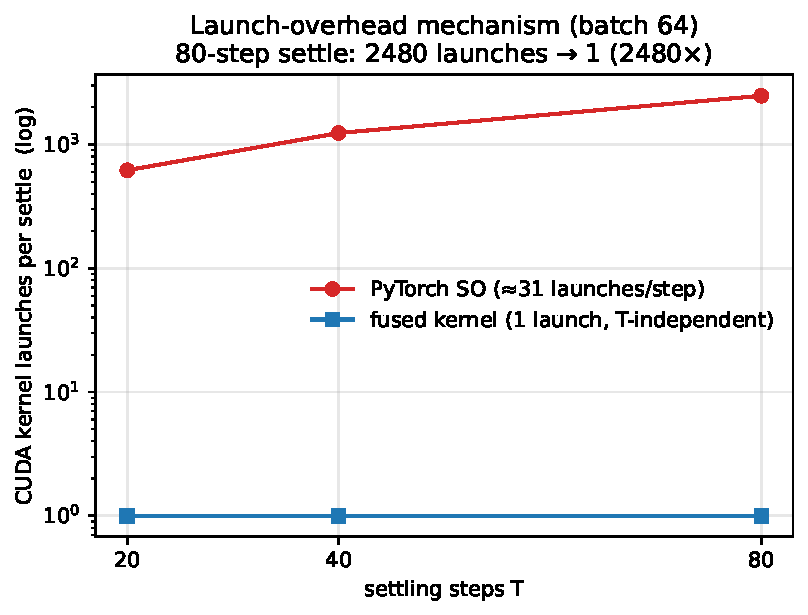
\includegraphics[width=0.8\linewidth]{fig4_launch_count}
  \caption{CUDA kernel launches per full settle versus the number of settling steps \(T\)
  (batch \(64\), RTX 3080 Ti). The PyTorch SO backend issues \(31\) launches per step
  (\(620\rightarrow1240\rightarrow2480\) for \(T=20,40,80\)); the fused kernel issues exactly one,
  independent of \(T\). This is the mechanistic confirmation that PC inference at this scale is
  launch-overhead-bound rather than compute-bound.}
  \label{fig:launch-count}
\end{figure}

Consistent with a launch-bound regime, the PyTorch SO settle costs roughly \SI{0.5}{\milli\second}
per step \emph{independent of batch size} from \(B=64\) up to \(B=4096\) (the per-step wall clock
barely moves while the work per step grows \(64\times\)), and the GPU is only \(\sim\!25\)--%
\SI{49}{\percent} utilised during the M4 runs. We note that this ``framework tax'' of many tiny
operator launches is a generic, previously documented phenomenon, not a discovery of this thesis;
the contribution is its quantification for PC inference and the kernel that removes it.

\subsection{Speedup and the architectural crossover}

\Cref{fig:kernel-speedup} plots the speedup of the fused kernel over the PyTorch backend versus
batch size for the topology \([784,256,256,10]\). The kernel wins decisively in the small-batch
regime, reaches break-even in the middle, and loses at large batch. With the final batch-tiling
and input-activation caching optimisations (v3), the measured behaviour is: \textbf{about
\(3.2\times\) at \(B=64\)}, \textbf{about \(2.0\times\) at \(B=256\)}, \textbf{break-even
(\(\sim\!1.0\times\)) around \(B=1024\)}, and a loss (\(\sim\!0.33\times\)) at \(B\ge 2048\). The
optimisation history is itself informative: the naive v1 kernel (one block per sample, each weight
re-read from global memory per sample) already gave \(3.2\times\) at \(B=64\) but lost
\(3\times\) at \(B=1024\) because it is bandwidth-limited; v2 processes a tile of \(8\) samples per
block and reuses each weight across the tile (the key GEMM optimisation); v3 additionally caches
the clamped --- and therefore constant --- \(\phi(\text{input})\) tile in shared memory, removing
\(\sim\!256\times\) redundant global reads of the first weight block. These optimisations moved the
crossover from \(\sim\!256\) to \(\sim\!1024\)--\(1500\).

\begin{figure}[t]
  \centering
  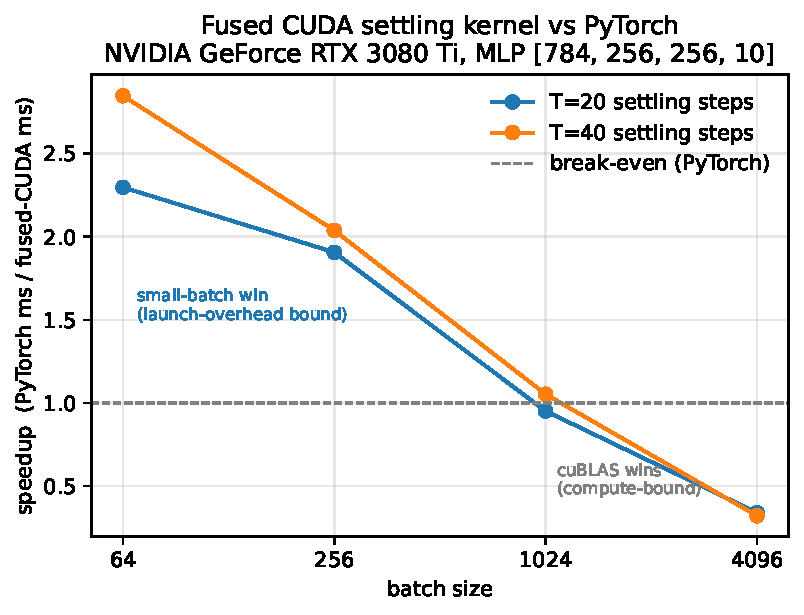
\includegraphics[width=0.8\linewidth]{fig1_kernel_speedup}
  \caption{Fused CUDA settling-kernel speedup over the PyTorch backend versus batch size
  (RTX 3080 Ti, MLP \([784,256,256,10]\), settling steps \(T=20\) and \(40\)). The kernel wins at
  small batch (launch-overhead bound, \(\sim\!3.2\times\) at \(B=64\), \(\sim\!2.0\times\) at
  \(B=256\)), reaches break-even around \(B\approx 1024\), and is outperformed by cuBLAS at
  \(B\ge 2048\), where the workload becomes compute-bound. The small/medium-batch regime is the
  one relevant to online and continual PC training.}
  \label{fig:kernel-speedup}
\end{figure}

The large-batch loss is not a tuning failure but a fundamental architectural trade-off, and we
report it as a positive systems finding rather than as ``not yet optimised''. At large batch the
workload becomes \emph{compute}-bound: the naive in-kernel GEMM uses scalar fused multiply-adds
with no register blocking and reaches only a fraction of the FLOP peak, whereas cuBLAS is
register-blocked and runs near optimum. Crucially, \textbf{the fused-resident design and a
cuBLAS-class GEMM are architecturally opposed}: keeping all \(T\) states resident in registers and
shared memory (which is what kills the launch overhead) consumes precisely the register and
shared-memory budget that a fast tiled GEMM would need. The two goals compete for the same scarce
resource. The honest conclusion is therefore that the fused kernel is the right tool in the
small-to-medium batch regime (\(B\lesssim 1024\), \(1\)--\(3\times\), the realistic MNIST-scale PC
training regime), and the PyTorch/cuBLAS backend is the right tool at \(B\ge 2048\); a fully
register-blocked tiled in-kernel GEMM would amount to re-implementing cuBLAS and is out of scope.

\subsection{Generality and in-study use}

Two facts elevate the kernel from a microbenchmark to a usable engine. First, it is no longer tied
to a fixed topology. The original kernel was specialised to two hidden layers (\texttt{model.n==3});
a \emph{general-depth} per-sample variant (\texttt{pcn\_settle\_so\_deep}) passes the per-layer
weights, states, and biases as arrays of device pointers (as \texttt{int64} addresses) with
shared-memory offsets computed at launch, and runs the same Jacobi update as the PyTorch backend
for arbitrary depth. It was validated to \(\sim\!10^{-6}\) (\texttt{allclose}) across depths
\(2\)--\(5\) (one to four hidden layers) \(\times\) \(\{\tanh,\text{sigmoid}\}\) \(\times\)
\(B\in\{32,256\}\) --- \textbf{all 16 configurations} matching the PyTorch equilibrium. (A Windows
portability trap was fixed in the process: \texttt{long} is 32-bit on MSVC, so the pointer arrays
must be typed \texttt{int64\_t}.) Second, the kernel was used as the \emph{backend of the project's
own Song-faithful study} (\Cref{sec:exp-song}), which runs at batch \(32\) --- exactly the
small-batch regime the kernel targets. On that real workload it delivers \textbf{\(1.45\times\)
end-to-end} wall-clock (\SI{103.9}{\second}\(\rightarrow\)\SI{71.6}{\second} at budget 800, ten
seeds) with \textbf{per-seed bit-identical results} (maximum accuracy difference \(0.00\) pp). The
modest \(1.45\times\) --- rather than the \(3.2\times\) of the \(B=64\) microbenchmark --- is
honest: the training loop gains in the small-batch regime, but evaluation settles at batch \(512\),
which dilutes the average. Integrating the kernel into the study also exposed and fixed a silent
activation bug (\texttt{sigmoid} had been mapped to \(\tanh\) internally), now guarded.

\subsection{Novelty scope}

To our knowledge this is the first hand-written, fused CUDA settling kernel \emph{for PC}. The
claim is bounded by a direct audit of eleven open PC libraries (none ship a \texttt{.cu} file; all
are JAX/JIT --- e.g.\ PCX \citep{pinchetti2024pcx}, JPC \citep{millidge2024jpc} --- or
PyTorch-autograd, e.g.\ PRECO \citep{vanzwol2024preco}) and, for double assurance, of the closest
algorithmic relative, the Equilibrium Propagation family \citep{scellier2017ep, laborieux2021ep},
which likewise ships no hand-written CUDA settling kernel (\Cref{ch:related}; \Cref{app:kernel}).
We are careful \emph{not} to claim the persistent, states-resident, single-launch \emph{technique}
as novel --- it is established prior art (Baidu/cuDNN persistent RNNs
\citep{diamos2016persistent}, recent LLM megakernels). The contribution is the transfer of that
technique to PC, plus the measurement.

\section{Fair PC versus BP}\label{sec:exp-pcbp}

This is the methodological heart of the thesis. The protocol (\Cref{sec:protocol}) holds the
architecture, the initialisation, the data, and --- critically --- the loss function fixed, so
that the \emph{only} variable is the learning rule; the learning rate is tuned per method on a
held-out validation split and \emph{reported} on test; every number is a mean over three seeds with
a \(68\%\) bootstrap CI. Under this protocol the headline result is null: PC is statistically
indistinguishable from loss-matched BP.

\subsection{A methodological prerequisite: tune \texorpdfstring{\(\eta_x\)}{eta\_x} and
\texorpdfstring{\(\eta_w\)}{eta\_w} jointly}

A non-obvious lesson preceded the fair numbers and is reportable in its own right. An early
comparison fixed the state learning rate at \(\eta_x=0.1\) and swept only the weight learning rate
\(\eta_w\); PC then appeared to lose by \(\sim\!10\) pp. A two-dimensional \(\eta_x\times\eta_w\)
scan revealed a \emph{stability frontier} coupling the two: at \(\eta_x=0.1\), PC \emph{diverges}
for \(\eta_w=0.05\) (collapsing to chance, \SI{9.8}{\percent}), whereas at the lower
\(\eta_x=0.05\) the same \(\eta_w=0.05\) is stable and reaches \SI{84.9}{\percent}. With joint
tuning (\(\eta_x=0.05,\ \eta_w=0.05\)) the apparent accuracy gap shrinks from \(\sim\!10\) to
\(\sim\!4\) pp. \textbf{Sweeping only \(\eta_w\) systematically handicaps PC}; the \(\sim\!10\) pp
was largely a tuning artifact. The state and weight learning rates must be tuned together.

\subsection{The confounded first results and their correction}

An adversarial methodology review (four critic agents) found that the project's initial
``PC wins'' were artifacts. Two confounds were identified at this stage and a third in the
class-incremental setting below.
\begin{itemize}
  \item \textbf{Confound 1 --- loss mismatch.} PC minimises MSE to a one-hot target, but the first
  BP baseline minimised cross-entropy (CE). That violates ``only the learning rule varies''. The
  fix is to add a \textbf{BP(MSE)} control arm with the \emph{identical} objective to PC. The fair
  comparison is \textbf{PC(MSE) vs BP(MSE)}; the quantity \(\text{BP(CE)}-\text{BP(MSE)}\) isolates
  the pure loss effect.
  \item \textbf{Confound 2 --- the plasticity confound.} In continual learning, ``forgets less''
  can simply mean ``learns each task less well''. The fix is to additionally measure learning
  accuracy (the diagonal of the accuracy matrix) and retained task-0 accuracy, so that retention
  is read against how much was actually learned.
\end{itemize}

\subsection{Bulk accuracy and noise robustness}

\Cref{fig:pc-vs-bp} shows the deconfounded comparison; the bulk numbers (\(10\)k training
examples, \(8\) epochs, \(T=40\), jointly tuned, three seeds) are:

\begin{table}[t]
  \centering
  \caption{Deconfounded bulk comparison on MNIST (10k examples, matched MSE loss unless noted;
  mean over 3 seeds with \(68\%\) bootstrap CI). The fair PC-vs-BP(MSE) gap is \(+0.4\) pp with
  overlapping CIs; the loss effect \(\text{BP(CE)}-\text{BP(MSE)}\) is \(+5.9\) pp.}
  \label{tab:bulk}
  \begin{tabular}{lcc}
    \toprule
    Arm & Test accuracy & Noise \(\sigma=1.0\) \\
    \midrule
    PC (MSE)                         & \(83.5\%\) \([82.8, 84.3]\) & \(52.6\%\) \\
    \textbf{BP (MSE)} --- fair arm   & \(83.9\%\) \([83.6, 84.3]\) & \(60.4\%\) \\
    BP (CE) --- reference            & \(89.9\%\) \([89.7, 90.0]\) & \(81.0\%\) \\
    \bottomrule
  \end{tabular}
\end{table}

The \textbf{fair gap PC(MSE) vs BP(MSE) is \(+0.40\) pp, and the CIs overlap} --- the two learning
rules are statistically indistinguishable. The \textbf{loss effect \(\text{BP(CE)}-\text{BP(MSE)}\)
is \(+5.92\) pp.} In other words, the naive ``BP beats PC by \(4\)--\(10\) pp'' that the literature
might lead one to expect is here \emph{almost entirely the loss function, not the learning rule}.
On noise robustness the story is similar in shape: BP(MSE) remains about \(8\) pp more robust than
PC(MSE) at \(\sigma=1.0\) (\(60.4\%\) vs \(52.6\%\)) --- a real but small effect, dwarfed by the
\(\sim\!28\) pp gap one would have wrongly attributed to PC's disadvantage had the comparison been
against BP(CE). A separate ablation confirmed that the settling budget is not hiding anything:
varying \(T\in\{20,40,80\}\) does not change bulk accuracy, ruling out an under-settling artifact.

\begin{figure}[t]
  \centering
  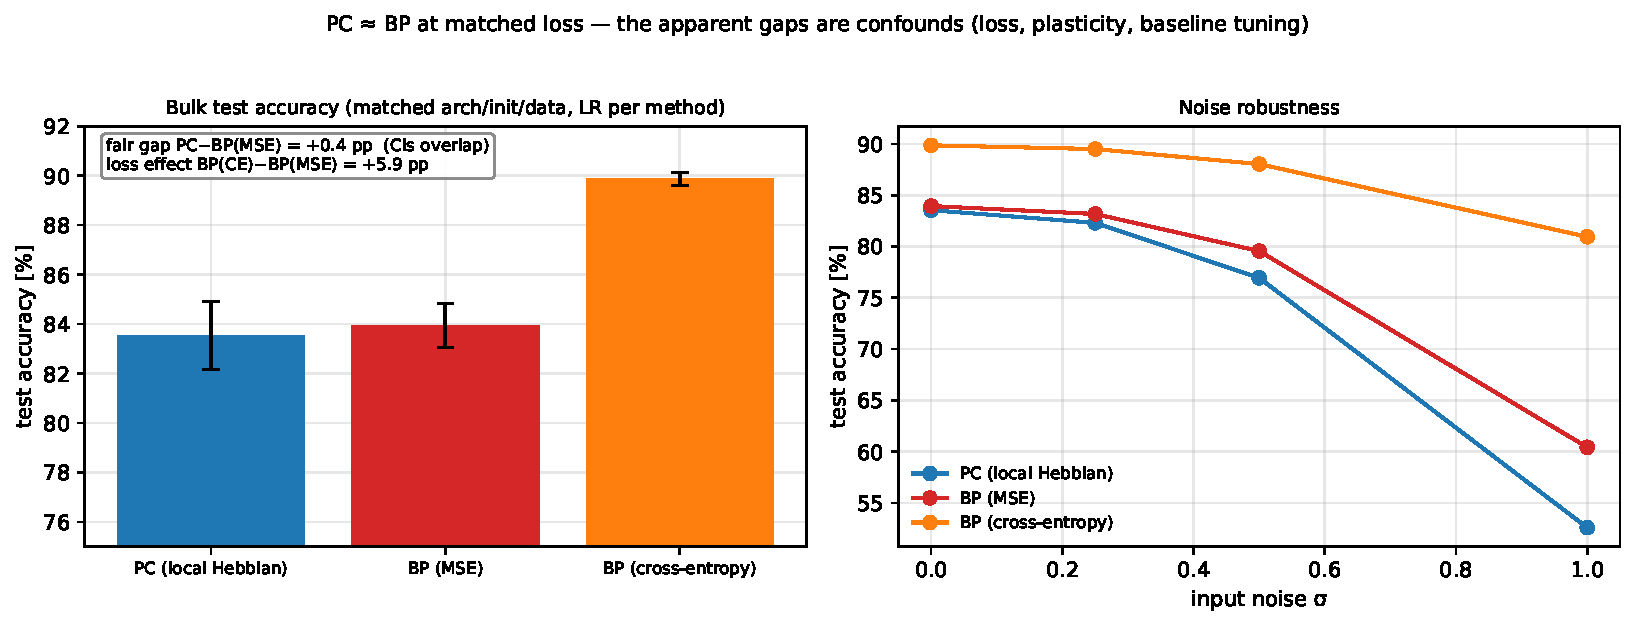
\includegraphics[width=0.95\linewidth]{fig2_pc_vs_bp}
  \caption{Matched-loss PC versus BP on MNIST (3 seeds, \(68\%\) bootstrap CIs). \emph{Left:} bulk
  test accuracy --- PC(MSE) and BP(MSE) are indistinguishable (CIs overlap); BP(CE) leads by the
  \(+5.9\) pp loss effect, not by the learning rule. \emph{Right:} test accuracy versus additive
  input-noise \(\sigma\) --- BP(MSE) is modestly more robust than PC(MSE), but the large naive gap
  is again mostly the loss function.}
  \label{fig:pc-vs-bp}
\end{figure}

\subsection{Continual learning: domain-incremental}

On Permuted-MNIST (five tasks, domain-incremental), against the fair BP(MSE) arm, the earlier
``PC forgets less'' headline collapses:

\begin{table}[t]
  \centering
  \caption{Permuted-MNIST domain-IL (5 tasks, matched loss; mean over 3 seeds, \(68\%\) CI on
  retained task-0). Against fair BP(MSE), BP forgets \emph{less} and learns each task better; the
  earlier ``PC forgets less'' was an artifact of comparing to BP(CE).}
  \label{tab:permuted}
  \begin{tabular}{lcccc}
    \toprule
    Arm & Final ACC & Learn ACC & BWT & Retained task-0 \\
    \midrule
    PC (MSE)         & \(55.0\%\) & \(65.1\%\) & \(-12.7\%\) & \(41.8\%\) \([39.8, 43.8]\) \\
    \textbf{BP (MSE)} & \(62.9\%\) & \(69.1\%\) & \(\mathbf{-7.8\%}\) & \(\mathbf{54.2\%}\) \([54.1, 54.3]\) \\
    BP (CE)          & \(60.7\%\) & \(78.7\%\) & \(-22.5\%\) & \(47.2\%\) \\
    \bottomrule
  \end{tabular}
\end{table}

The headline was \emph{doubly} artifactual. (1) It compared against BP(CE), which forgets more
because of aggressive softmax updates; against the fair BP(MSE), BP forgets \emph{less}
(\(-7.8\%\) vs \(-12.7\%\)). (2) PC learns each task less well (learning accuracy \(65.1\%\) vs
\(69.1\%\)) and retains task-0 \emph{absolutely} worse (\(41.8\%\) vs \(54.2\%\), disjoint CIs) ---
the plasticity confound. The decision is therefore \emph{not proven}.

\subsection{Continual learning: class-incremental (Song's regime)}

The class-incremental setting (Split-FashionMNIST, two tasks of five classes; Split-MNIST, five
tasks of two classes), with the BP learning rate tuned per arm by learning accuracy, is where a
third confound surfaced:

\begin{table}[t]
  \centering
  \caption{Class-IL parity (mean over 3 seeds, \(68\%\) CI on retained task-0). Against a correctly
  tuned, \emph{learning} BP(MSE) baseline, PC shows no advantage in either split.}
  \label{tab:classil}
  \begin{tabular}{llccccc}
    \toprule
    Setup & Arm & Final ACC & Learn ACC & BWT & Retained T0 & Decision \\
    \midrule
    \multirow{2}{*}{Split-FashionMNIST (2\(\times\)5)}
      & PC      & \(60.9\%\) & \(84.3\%\) & \(-46.8\%\) & \(37.8\%\) \([34.3,41.3]\) & \\
      & BP(MSE) & \(61.3\%\) & \(86.1\%\) & \(-49.6\%\) & \(37.3\%\) \([34.0,40.6]\) & \textbf{NO (all overlap)} \\
    \midrule
    \multirow{2}{*}{Split-MNIST (5\(\times\)2)}
      & PC      & \(70.8\%\) & \(97.4\%\) & \(-33.3\%\) & \(60.1\%\) \([58.6,61.7]\) & \\
      & BP(MSE) & \(73.4\%\) & \(97.5\%\) & \(-30.2\%\) & \(62.0\%\) \([60.4,63.7]\) & \textbf{NO (BP marginally better)} \\
    \bottomrule
  \end{tabular}
\end{table}

Even in Song's own class-IL interference regime, against a correctly tuned, \emph{learning} BP(MSE),
there is \textbf{no PC advantage}: PC and BP(MSE) are statistically indistinguishable on
Split-FashionMNIST, and BP is marginally better on Split-MNIST. The third confound is the
\textbf{untuned-baseline confound}: an untuned BP(MSE) (\(\eta_w=0.1\)) stalls at chance
(\(\sim\!50\%\)) on Split-MNIST, manufacturing a false PC ``win'' that the learning-accuracy
diagnostic caught. What remains is a consistent stability--plasticity trade-off --- BP(CE) learns
the most and forgets the most, PC learns the least and forgets the least --- but PC sits
\emph{on the same curve} as loss-matched BP, not above it.

\subsection{Synthesis: three confounds, one null}

Across every tested regime (bulk accuracy, noise, sample efficiency, Permuted-MNIST domain-IL,
Split-FashionMNIST and Split-MNIST class-IL), with matched loss and fairly tuned baselines,
\textbf{vanilla SO-PC shows no advantage over BP} --- on par in accuracy and learning, on the same
stability--plasticity curve, slightly worse under noise. All three previously observed ``PC wins''
were methodological artifacts. The scientific value, as argued in \Cref{ch:discussion}, is a clean
null result \emph{plus} the systematic exposure of three confounds --- the loss function, the
plasticity confound in forgetting metrics, and an untuned baseline learning rate --- that bias
naive PC-vs-BP comparisons. We stress what this does \emph{not} mean: it does not globally refute
\citet{song2024prospective}, whose setup differs in training schedule, activation, width, and
possibly metrics. The defensible claim is bounded: \emph{at MNIST/FashionMNIST scale with a fairly
tuned BP baseline, the PC advantage disappears.} The strongest test of that boundary --- a faithful
replication of Song's exact protocol --- is the subject of the next section.

\section{Architecture-Faithful Replication of Song's Exact Protocol}\label{sec:exp-song}

The class-IL results above follow Song's \emph{regime} but not his exact training. To probe whether
the null survives a strict replication, we built the most architecture-faithful reproduction of
\citet{song2024prospective} we could, and we use it to illustrate how an adversarial verification
caught a premature finding before it reached the writeup.

\subsection{What was built}

The setup (\texttt{run\_alternating}) pits two disjoint five-class tasks from FashionMNIST against
each other, sharing a \emph{single} five-output head (which forces interference), trained by
\textbf{minibatch-level alternation} (\texttt{swap\_every=4} updates, then switch task; batch
\(32\)). The network is \([784,32,32,5]\) with \textbf{sigmoid} activations and
\textbf{Xavier-normal} initialisation. Checked against Song's Methods section, this matches on the
faithful axes: four layers, \(32\) hidden units per layer, sigmoid, Xavier, two disjoint
five-class tasks, shared head, alternating training --- in contrast to the \Cref{sec:exp-pcbp}
proxy, which was sequential, \(\tanh\), and \([256,256]\).

\subsection{The framing correction (an adversarial three-lens review)}

Three independent verification lenses --- literature faithfulness, statistics, and
alternative-explanations --- dismantled the first draft of this experiment; all three corrections
are folded in. The most important is the \textbf{framing correction} from the literature lens.
Song's Fig.~4e is \emph{not} a ``PC is robust across learning rates'' claim (that is his Fig.~3,
on target alignment). Fig.~4e shows \emph{less catastrophic interference}, with the learning rate
optimised \emph{separately per method} (its caption plots the mean test error of both tasks versus
learning rate). We had initially misattributed it as a learning-rate-robustness claim. The
corrected experiment therefore tests \emph{interference} (not LR robustness), tunes the learning
rate per method, and reports the worse of the two tasks' accuracies (\emph{min-both}) as the true
interference tell alongside Song's mean-both metric. This misframing-then-correction is itself a
reusable safeguard, discussed in \Cref{ch:discussion}.

\subsection{Budget as a controlled axis}

A faithfulness-versus-trainability tension appeared: Song's \emph{exact} budget (\(\sim\!84\)
minibatch iterations, swapping every \(4\)) leaves \emph{every} method at chance in our hands (all
arms \(\sim\!20\)--\(30\%\) at a chance level of \(20\%\)). Rather than silently enlarge the budget,
we make it a \textbf{controlled axis}: \(84\) (exact) \(\rightarrow\) \(250\) \(\rightarrow\) \(800\)
\(\rightarrow\) \(2500\) (convergence), and report the whole curve.

\subsection{Results}

\Cref{fig:budget-sweep} and \Cref{tab:budget} report the ten-seed sweep, run on the fused CUDA
kernel (per-seed identical to PyTorch, which doubles as a practical test of the kernel
integration). The metric \emph{min-both} --- the weaker of the two tasks --- is the genuine
interference indicator; \emph{mean-both} is Song's reported metric. The learning rate was tuned per
method (it landed at \(0.1\) at the trainable budgets).

\begin{table}[t]
  \centering
  \caption{Song-exact alternating Split-FashionMNIST, ten seeds. Mean-both and worse-task min-both
  accuracy (\%) with \(\pm 1\sigma\) bootstrap intervals; \(\Delta\)min is PC \(-\) BP(MSE). At
  \emph{no} budget does the PC-vs-BP(MSE) gap exceed \(1\sigma\) (the seed spread \(\sigma\) is
  \(\sim\!4\)--\(11\) pp on each arm). The pattern is directional only.}
  \label{tab:budget}
  \begin{tabular}{lcccc}
    \toprule
    Budget (iters) & \textbf{PC} mean/min & \textbf{BP(MSE)} mean/min & BP(CE) mean/min & \(\Delta\)min \\
    \midrule
    \textbf{84} (Song exact)   & \(26.6\,/\,24.8\) & \(28.0\,/\,26.2\) & \(29.6\,/\,27.9\) & \(-1.5\) \\
    250                        & \(39.2\,/\,36.2\) & \(38.4\,/\,34.7\) & \(41.0\,/\,36.3\) & \(+1.5\) \\
    800                        & \(64.1\,/\,55.8\) & \(50.6\,/\,44.8\) & \(58.4\,/\,49.8\) & \(+11.0\) \\
    \textbf{2500} (converged)  & \(73.6\,/\,68.9\) & \(68.5\,/\,63.2\) & \(74.3\,/\,69.6\) & \(+5.7\) \\
    \bottomrule
  \end{tabular}
\end{table}

\begin{figure}[t]
  \centering
  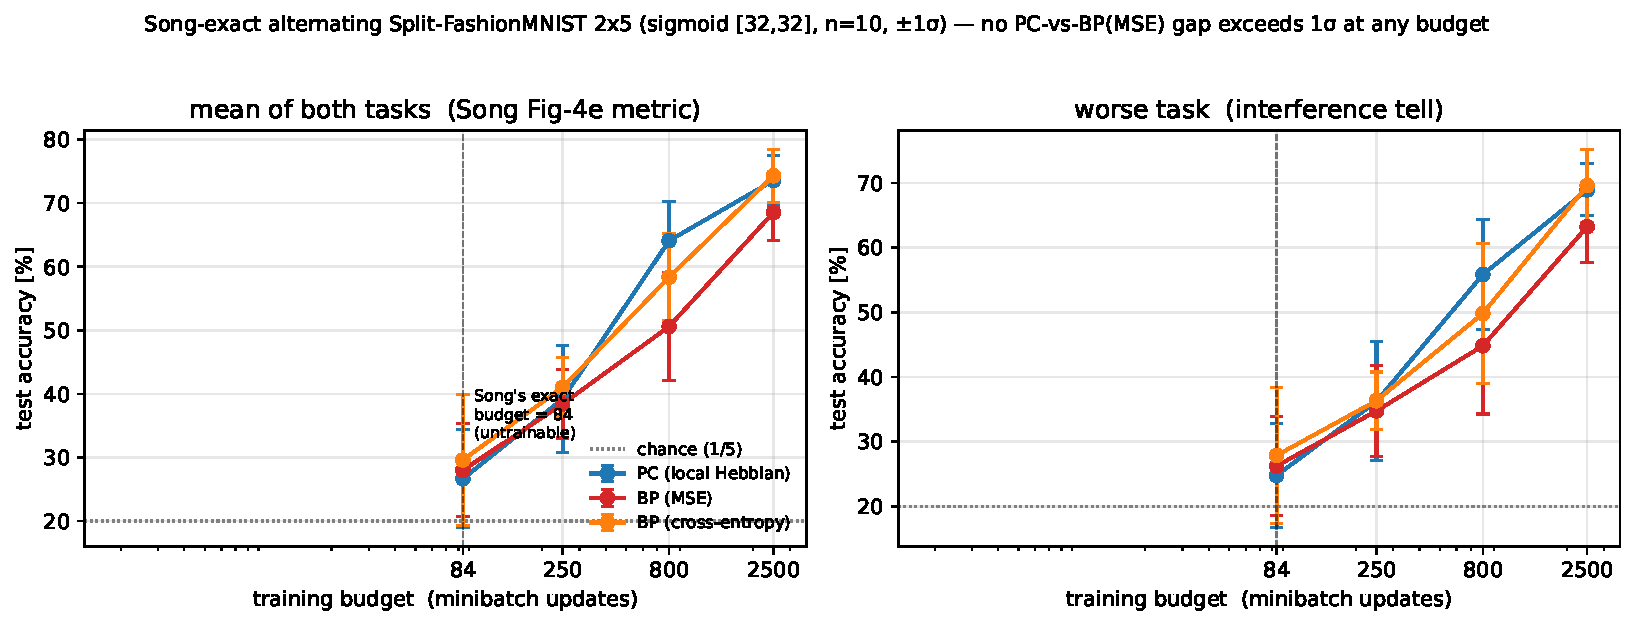
\includegraphics[width=0.95\linewidth]{fig3_alternating_budget_sweep}
  \caption{Song-exact alternating Split-FashionMNIST: mean-both (Song's metric) and worse-task
  min-both (interference tell) accuracy versus training budget (\(n=10\), \(\pm 1\sigma\)). No
  PC-vs-BP(MSE) gap exceeds \(1\sigma\) at any budget. PC learns slower early and pulls marginally
  ahead by convergence, but the gap stays inside the (large) seed spread; raising the seed count
  from five to ten did not make it significant. BP(CE) leads throughout --- the same loss confound
  as \Cref{sec:exp-pcbp}.}
  \label{fig:budget-sweep}
\end{figure}

\textbf{Verdict (calibrated): at \(n=10\) no PC-vs-BP(MSE) difference is separated by \(\ge1\sigma\)
at any budget.} The per-arm seed spread (\(\sigma\approx 4\)--\(11\) pp) is large relative to every
point-estimate gap, so the effects are \emph{directional, not significant}. The direction is
consistent and worth recording: PC learns \emph{slower early} (at budgets 84 and 250 it trails
BP(MSE) by a few points --- settling needs more steps to reach the ``prospective configuration''),
then \emph{catches up and edges marginally ahead by convergence}. At the converged budget of 2500
the point estimates favour PC by \(+5.0\) pp mean-both and \(+5.7\) pp min-both; at budget 800 the
point gap is even larger (\(+13.5\) and \(+11.0\) pp) but the spread there is enormous
(\(\sigma_{\text{sum}}\sim9\)--\(16\) pp), so any single-budget claim is noise. Notably the
min-both edge equals or exceeds the mean-both edge, a \emph{weak} hint that PC balances the two
tasks slightly better --- but it is inside the noise. BP(CE) leads throughout (the same loss
confound), so it carries no information about the learning rule.

This is the \emph{first} regime in which vanilla PC does not sit \emph{behind} loss-matched BP at
the convergence point (in \Cref{sec:exp-pcbp} PC was on par to slightly behind). It neither refutes
Song (different budget semantics and scale) nor confirms him (the effect is not separable from
zero). The honest conclusion: the faithful replication reproduces no clear PC interference
advantage at ten seeds, consistent with the overall ``PC \(\approx\) BP under fair tuning''
verdict. We also record the disclosed deviations from Song: a fixed \(T=20\) (no convergence
tolerance, so under-settling may co-explain PC's early slowness), and the budget itself (Song's 84
iterations are untrainable in our hands). The statistics lens additionally corrected a labelling
slip in an earlier intermediate report: the intervals are \(68\%\) (one-\(\sigma\)) à la Song, not
\(95\%\).

\subsection{Why the kernel matters here}

This section is the regime \emph{for which} the fused settling kernel was planned: PC settling at
batch \(32\) is launch-overhead-bound (\Cref{sec:exp-kernel}), exactly what the kernel removes. Run
end-to-end on the real budget-800 workload, the kernel gives the \(1.45\times\) reported above at
per-seed-identical results. This is the concrete link between the systems contribution (Hook~A) and
the science contribution (Hook~B): the hand-written kernel is the engine of a real study, not a
benchmark artifact.

\section{Generative Predictive Coding}\label{sec:exp-gen}

This section demonstrates PC's distinctive ``one mechanism, many tasks'' property --- and, equally
honestly, shows that it only appears when the model is \emph{generatively} trained.

\subsection{A discriminative PC cannot generate}

On the discriminatively trained network (test accuracy \(90.6\%\)), running the same settling
machinery ``backwards'' fails by construction. Clamping a label and settling the input yields grey
noise, not a recognisable digit; inpainting an occluded half preserves the visible pixels exactly
but fills the occluded region with noise; and OOD detection by residual energy gives an AUC of only
\(0.438\) against uniform-noise OOD --- no separation. This is architectural, not a tuning failure.
The discriminative PC clamps input \emph{and} label and settles only the hidden states with a
feedforward-predictive structure (\(\text{pred}_{i+1}=W_i\,\phi(s_i)+b_i\)); it learns an
input\(\rightarrow\)label map, not a generative model of the inputs. There is no learned image
manifold for ``backward'' settling to find, and with the input clamped the free states can always
relax to the zero-energy feedforward solution, so residual energy cannot separate OOD.

\subsection{A generative PC delivers the full capability set}

Reversing the orientation to \([10,256,256,784]\) (label\(\rightarrow\)image) and training
\emph{generatively} (clamp the label at the input and the image at the output, settle the hidden
states, apply the local Hebbian update --- the same \texttt{PCN}, \texttt{settle}, and
\texttt{weight\_update}) yields a generative model. The results (\(30\)k images, \(10\) epochs,
GPU; \texttt{scripts/demo\_generative\_v2.py}) are summarised in \Cref{tab:generative}.

\begin{table}[t]
  \centering
  \caption{The same settling rule, two training orientations. Generative PC recovers the
  capabilities a discriminative PC cannot provide.}
  \label{tab:generative}
  \begin{tabular}{lll}
    \toprule
    Capability & Discriminative (§\ref{sec:exp-gen}) & \textbf{Generative} \\
    \midrule
    Generation (clamp label \(\rightarrow\) image) & grey noise & recognisable per-class prototypes 0--9 \\
    Inpainting (fill occluded half)                & noise fill & structured (blurry) reconstruction \\
    Anomaly (MNIST vs uniform OOD)                 & AUC \(0.44\) & \textbf{AUC \(1.00\)} \\
    \bottomrule
  \end{tabular}
\end{table}

The generative model produces \textbf{recognisable per-class digit prototypes}, reconstructs
occluded halves with structured (if blurry) content, and separates uniform-noise OOD with a perfect
\textbf{anomaly AUC of \(1.00\)} (in-distribution residual energy \(5.1\) versus OOD \(94.5\)). The
same settling mechanism, varying only what is clamped, classifies, generates, inpaints, and detects
anomalies. A stability finding is reportable on its own: the \(784\)-dimensional output makes the
hidden-settling gradient (\(\varepsilon_{\text{out}}@W\)) about \(\sqrt{784}\approx28\times\) larger
than for the \(10\)-dimensional label head, so a state learning rate of \(0.1\) (fine for the
discriminative model) diverges to NaN; the state LR must scale as \(\sim\!1/\sqrt{\text{output-dim}}\)
(\(\eta_x\approx0.01\)) for stable settling.

The honest caveats temper the win. A one-hot input produces only ten distinct outputs, so these are
\emph{class prototypes} (the per-class mean), not diverse samples; diversity would require a
continuous latent with a prior (VAE-style). Inpainting is prototype-driven, hence blurry rather than
pixel-sharp. And uniform noise is an \emph{easy} OOD, so AUC \(1.0\) is not a hard test; a near-OOD
such as FashionMNIST or rotated digits would be the harder next step. The interpretive significance
of the discriminative/generative distinction is taken up in \Cref{ch:discussion}.

\section{Optional Extensions: iPC and EWC}\label{sec:exp-depth}

Two further variants were implemented \emph{and} validated, each tightening a loose end. They are
optional depth rather than headline results.

\subsection{Incremental PC (iPC)}

Incremental PC \citep{salvatori2024ipc} (\texttt{update\_variant="ipc"}) interleaves a weight
update with \emph{every} settling step, rather than settling fully and updating once at
equilibrium. A correctness anchor pins it to the standard rule: with \(\eta_w=0\), one iPC step
reproduces a standard settling step \emph{exactly} (iPC's state update \emph{is} the SO update; it
merely also moves the weights). The empirical finding is that \textbf{iPC is markedly more
learning-rate-sensitive}: because it applies \(T\) weight updates per minibatch, its effective
weight LR is \(\sim\!T\times\) larger, and at the standard \(\eta_w=0.02\) it diverges (NaN). At a
\(\sim\!T\times\)-smaller rate (\(\eta_w\approx0.005\), i.e.\ \(\sim\!\eta_w/T\)) it is stable and,
in a fast-training regime (MNIST, \(3\)k samples, \(2\) epochs), reaches \textbf{\(74.3\%\) versus
\(63.1\%\) for standard PC} --- iPC learns faster per step, consistent with
\citet{salvatori2024ipc}. The lesson: iPC trades learning-rate sensitivity for faster per-step
learning, and needs a \(\sim\!T\times\)-smaller weight LR to be competitive.

\subsection{EWC as a continual-learning positive control}

Elastic Weight Consolidation \citep{kirkpatrick2017ewc} was added as a third class-IL arm
(\texttt{run\_class\_il(method="ewc")}): after each task the diagonal empirical Fisher (mean squared
gradients) and the optimal weights are stored, and later tasks carry the quadratic anchor
\((\lambda/2)\sum_i F_i(\theta_i-\theta_i^\ast)^2\). Validated end-to-end on Split-MNIST
(\(5\times2\), in a \emph{learning} regime), EWC \textbf{forgets less than the matched BP(MSE)}:
\textbf{BWT \(-41.1\%\) vs \(-45.7\%\)}, \textbf{final accuracy \(65.7\%\) vs \(62.0\%\)}, at equal
learning (learning accuracy \(98.5\%\)). This is exactly the expected EWC effect and serves as a
\emph{positive control}: it confirms the continual-learning harness measures forgetting correctly.
(Consistent with the \Cref{sec:exp-pcbp} lesson, in a too-weak regime --- where BP is stuck at
chance --- EWC is inert, because there is nothing learned to forget.)

\section{Autonomous Hyperparameter Search}\label{sec:exp-search}

The final experiment is an internal consistency check rather than a discovery. A bounded random
search over \((T, \eta_x, \eta_w)\), implemented as a thin layer over the \texttt{train\_and\_eval}
interface (\Cref{ch:method}), independently rediscovers the \(\eta_x\leftrightarrow\eta_w\)
interaction surfaced manually in \Cref{sec:exp-pcbp}. The best configuration in the run prefers a
\emph{low} state learning rate, a \emph{high} weight learning rate, and a \emph{high} settling
budget (\(\eta_x=0.02\), \(\eta_w=0.05\), \(T=40\), reaching \(77.6\%\) on the short MNIST run in
\texttt{results/m7\_search.json}), where the high \(\eta_w\) is only stable \emph{because} \(\eta_x\)
is low --- precisely the stability frontier identified by hand. The search also records
\texttt{settling\_steps\_to\_converge} per configuration (e.g.\ \(94\) steps at the
high-\(\eta_w\)/low-\(\eta_x\) optimum versus \(\sim\!30\) at the more aggressive settings),
confirming that the better-learning regime is also the slower-settling one. That an automated search
re-derives a manually found coupling is a small but reassuring validation that the
hyperparameter landscape was characterised correctly, and that the \texttt{train\_and\_eval}
contract is sound.

\bigskip

\noindent\textbf{Chapter summary.} The fused kernel is a real but bounded engineering win
(\(3.2\times\) at small batch, an architectural crossover at large batch), the first of its kind for
PC and now general-depth and used as the engine of a real study. The fair PC-vs-BP comparison is a
clean null --- PC \(\approx\) BP at matched loss across every regime tested --- plus the exposure of
three confounds; the Song-faithful replication, at ten seeds, finds no \(\ge1\sigma\) gap at any
budget. A generatively trained PC recovers the ``one mechanism, many tasks'' property that a
discriminative PC cannot. We interpret these results, and what they mean for the field, in
\Cref{ch:discussion}, and bound them in \Cref{ch:limitations}.

\chapter{Discussion}\label{ch:discussion}

The preceding chapter reported what we measured. This chapter asks what those measurements
\emph{mean}. We are deliberately careful here, because the central findings of this study are
largely null --- under a fair comparison, our from-scratch State-Optimization predictive coding
(PC) network neither beats nor is beaten by backpropagation (BP) at MNIST/FashionMNIST scale ---
and a null result is precisely the kind of result that invites overinterpretation in both
directions. We therefore separate four distinct interpretive questions and treat each on its own
terms: whether PC's reputed advantages are real (\Cref{sec:disc-real}), why a single methodological
checklist explains the literature's disagreement and transfers beyond PC
(\Cref{sec:disc-checklist}), what the systems measurements teach us about \emph{where the compute
actually goes} in PC inference (\Cref{sec:disc-systems}), what a generative PC genuinely buys that a
discriminative one does not (\Cref{sec:disc-generative}), and how an adversarial-verification habit
caught a framing error before it reached the page (\Cref{sec:disc-adversarial}). We close with an
explicit accounting of threats to the validity of the inferences drawn here
(\Cref{sec:disc-threats}). Throughout, the substantive enumeration of what this study \emph{cannot}
claim is deferred to \Cref{ch:limitations}; the present chapter is about interpretation, not
caveats.

\section{Are Predictive Coding's Advantages Real?}\label{sec:disc-real}

Predictive coding is advertised in the literature as a local-learning alternative to
backpropagation that, beyond its biological plausibility, is empirically \emph{better} along
several axes: it is said to approximate BP's gradients while needing fewer samples, to forget less
in continual-learning settings, to be more robust, and to do all of this with a single settling
mechanism that also doubles as a generative model. Our fair-comparison study
(\Cref{sec:exp-pcbp,sec:exp-song}) found none of the discriminative-side advantages to survive once
the comparison is made honestly. The headline verdict is parity: at matched loss, with
per-method-tuned learning rates and bootstrap confidence intervals over multiple seeds, PC and BP
are statistically indistinguishable on bulk accuracy, the confidence intervals overlap, and the
directional residue --- slightly worse noise robustness for PC, a hair's-breadth edge in the
faithful interference replication --- never exceeds one standard deviation.

\subsection{What ``parity'' does and does not mean}

It is worth stating the verdict with care, because ``PC $\approx$ BP'' is easy to misread. We are
\emph{not} claiming that PC and BP are the same algorithm. They are demonstrably not: PC settles the
free states to a (near-)equilibrium before touching the weights, whereas BP computes a single
backward pass and updates immediately, and the two procedures produce genuinely different
intermediate activity (this is the substance of Song et al.'s ``prospective configuration''
argument, \citealp{song2024prospective}). What we are claiming is narrower and more defensible:
along the \emph{outcome} metrics we measured --- test accuracy, noise robustness, sample efficiency,
and forgetting in continual learning --- the distinction between the two learning rules does not
manifest as a measurable performance gap once confounds are removed. The two rules arrive at
comparable solutions by different routes. That a different mechanism reaches the same place is itself
informative; it does not license the stronger claim that the mechanisms are equivalent, only the
claim that, at this scale and on these tasks, the mechanism does not buy a performance advantage.

Equally, parity is a \emph{scoped} claim, not a universal one. Our measurements live at
MNIST/FashionMNIST scale with shallow (two-to-five-layer) networks. The honest statement is that at
this scale, against a fairly tuned baseline, no PC advantage exceeds noise --- not that no advantage
can exist anywhere. The regimes in which PC is most strongly theorized to differ --- deep networks
where the prospective-configuration argument compounds across layers, genuine online single-example
streams, reinforcement learning --- are exactly the regimes our setup does not stress. This is the
correct frontier to defer to (\Cref{ch:limitations}), and we are careful not to overclaim past it.

\subsection{Why the literature disagrees}

If PC's advantages are not real at this scale, why does so much of the literature report them? Our
answer, and one of the transferable contributions of this study, is that the inconsistency is not
mysterious: naive comparisons trip over a small number of recurring confounds, and each confound
manufactures a spurious PC advantage in a predictable direction. We identified three (developed in
\Cref{sec:disc-checklist}), and in our own pre-confound runs all three fired. Our first
PC-versus-BP table showed an apparent BP \emph{win} on bulk accuracy and an apparent PC \emph{win}
on continual learning; the adversarial methodology review showed both to be artifacts. The bulk gap
was almost entirely the loss function --- cross-entropy versus mean-squared error to a one-hot
target --- not the learning rule, since the loss effect alone (BP-CE minus BP-MSE) accounts for the
bulk of a naive ``BP beats PC'' gap. The continual-learning gap was a double artifact: comparing
against a cross-entropy baseline (which forgets more because softmax produces large, aggressive
output updates) \emph{and} reading the forgetting metric without controlling for the fact that PC
learns each task less well in the first place, so it has mechanically less to forget.

This reframing reconciles what looks like a contradiction in the background literature. On the one
hand, a line of theoretical work shows that PC \emph{approximates} BP under restrictive conditions
--- the fixed-prediction regime of \citet{whittington2017approximation}, the arbitrary-graph result
of \citet{millidge2022backprop}, and the limiting analyses of \citet{innocenti2026limits}. On the
other hand, \citet{song2024prospective} argue that \emph{without} those constraints, energy-based
networks follow a distinct prospective-configuration dynamics that yields advantages. Both can be
true: PC collapses toward BP in the small-step, near-feedforward-initialization limit, and departs
from it when the settling is allowed to run to genuine equilibrium. Our finding sits on top of this:
even in the unconstrained, fully-settled regime where PC \emph{should} differ most, the difference
does not translate into a measurable advantage over a \emph{fairly tuned, loss-matched} BP at our
scale. The literature's disagreement is, on this reading, less about PC's true behaviour and more
about how carefully the BP baseline was constructed.

\section{The Confound Checklist as a Transferable Contribution}\label{sec:disc-checklist}

The most reusable product of this study is not the parity verdict itself but the diagnostic
machinery that produced it. We distilled the failure modes of naive PC-versus-BP comparisons into a
three-item checklist. We argue that this checklist is the genuine contribution of the methodological
strand of the thesis, because it generalizes well beyond PC: it applies to \emph{any} comparison
between a biologically-motivated learning rule and backpropagation, and indeed to many
``alternative-versus-baseline'' empirical claims in machine learning.

\subsection{The three confounds}

\paragraph{Confound 1: the loss function.}
The single largest hidden variable is the objective being minimized. A PC network that clamps a
one-hot target onto its linear output state and minimizes squared prediction error is minimizing
mean-squared error (MSE); a BP baseline that minimizes \texttt{CrossEntropyLoss} on logits is
optimizing a different loss surface entirely. These are not interchangeable: softmax cross-entropy
is well known to outperform MSE-to-one-hot on classification. Comparing PC-MSE against BP-CE
therefore conflates the learning rule with the loss, and because the loss effect is large
(\Cref{sec:exp-pcbp}), most of a naive gap is the objective, not the mechanism. The fix is to add a
matched BP-MSE arm so that the valid like-for-like comparison is PC-MSE versus BP-MSE, while the
difference BP-CE minus BP-MSE quantifies, and quarantines, the pure loss effect.

\paragraph{Confound 2: the stability--plasticity trade-off.}
In continual learning, ``forgets less'' is not the same as ``retains better.'' Backward transfer
measures the drop in accuracy relative to the freshly-learned diagonal; a model that writes weaker,
more diffuse task representations has a lower diagonal and therefore mechanically less to lose,
yielding a less-negative backward-transfer score that flatters it. A forgetting claim is only
defensible when read jointly against two controls: the per-task learn-accuracy (the diagonal, i.e.
how well each task was acquired) and the retained absolute accuracy on the first task after all
tasks (the sharpest single control, because it sidesteps the diagonal entirely). If PC ``forgets
less'' only because it learns less, the apparent advantage is a relabelling of underfitting.

\paragraph{Confound 3: the untuned baseline.}
A comparison is only as honest as its weakest baseline. We found that an untuned BP-MSE baseline
could sit stuck at chance on a class-incremental split, manufacturing a false PC ``win'' that a
learn-accuracy gate immediately exposed. The discipline this enforces is twofold: the baseline's
learning rate must be tuned on the same objective and validation protocol as the method under test,
and PC's own state and weight learning rates ($\eta_x$ and $\eta_w$) must be tuned \emph{jointly},
because they are coupled by a stability frontier --- sweeping $\eta_w$ alone, at a fixed and
too-large $\eta_x$, drives PC into divergence and systematically understates it.

\subsection{Why the checklist transfers}

None of these three confounds is specific to predictive coding. The loss confound bites whenever two
methods are compared under different objectives; the plasticity confound bites whenever a retention
metric is read without a learning control; the baseline confound bites whenever the comparison point
is left untuned. The checklist is thus a lightweight, reusable instrument for reviewers and authors
in an empirically confounded subfield: before believing a ``method X beats backpropagation'' claim,
ask whether the loss was matched, whether the retention metric was controlled for plasticity, and
whether the baseline was actually tuned to learn. We offer it in that spirit --- as a portable
artifact of the methodology, more durable than any single number in \Cref{ch:experiments}.

\section{The Systems Insight: Launch Overhead and the GEMM Trade-off}\label{sec:disc-systems}

The systems strand of the thesis produced the project's only unambiguous ``better'' result --- an
engineering win --- and it carries an interpretation worth drawing out independently of the speedup
figures. The measurement, not the speedup, is the contribution.

\subsection{PC inference is launch-overhead-bound, and that is a framework tax}

The headline systems observation (\Cref{sec:exp-kernel}) is that the PyTorch State-Optimization
backend spends roughly half a millisecond per settling step \emph{independent of batch size}, with
the GPU only partially utilized. The mechanistic evidence is direct: a launch-count profile shows
the PyTorch backend issuing thirty-one kernel launches per settling step (scaling linearly with the
number of settling steps $T$), whereas the fused kernel issues exactly one regardless of $T$. The
correct interpretation is that, at MNIST scale, PC inference is \emph{not} compute-bound; it is
bound by kernel-launch overhead --- the cost of dispatching many tiny operations from the host. This
is a recognized ``framework tax'' on workloads built from many small operations, and we are careful
to claim neither the observation nor the remedy as novel in general. The fused, persistent,
states-resident single-launch technique is established prior art, originating in cuDNN's persistent
RNN and Baidu's \texttt{persistent-rnn} \citep{diamos2016persistent} and reappearing in recent LLM
megakernels. What \emph{is} new, to our knowledge, is the transfer of that technique to the PC
settling loop and the measurement that pins the bottleneck: an audit of eleven open PC libraries and
the entire Equilibrium-Propagation family found none shipping a hand-written CUDA settling kernel
(\Cref{ch:related}; the audit is the substance of the novelty claim). The defensible statement is
therefore narrow --- ``first hand-written fused CUDA settling kernel \emph{for PC}, to our
knowledge'' --- and we hold it at that width deliberately.

\subsection{The architectural trade-off bounds the win}

The more interesting systems insight is \emph{why} the kernel wins only in a bounded regime. At
small and medium batch, fusing the $T$-step loop into one launch eliminates the launch overhead and
delivers a real speedup. But at large batch the bottleneck shifts from launch overhead to raw
compute, and here the design that wins at small batch actively works against you. A fused-resident
kernel holds the layer states on-chip across all $T$ steps; that residency consumes precisely the
register and shared-memory budget that a fast, register-blocked general matrix-multiply (GEMM) needs
to approach the hardware's floating-point peak. The fused-resident design and a cuBLAS-class GEMM are
thus \emph{architecturally opposed}: you cannot have both maximal residency and maximal GEMM
throughput in the same kernel, so at large batch the vendor library's register-blocked GEMM wins and
our naive in-kernel GEMM cannot keep up. This is not merely ``not yet optimized''; it is a structural
trade-off, and recognizing it as such is itself a reportable finding. Batch-tiling and caching the
clamped input activation push the crossover outward, but they do not abolish the trade-off.

\subsection{Why this matters for PC specifically}

The trade-off is not a defect for PC's purposes, because the regime where the kernel wins ---
small-to-medium batch --- is exactly the regime PC most naturally inhabits. PC is biologically
motivated as an online or near-online learner, and the prospective-configuration advantages are
theorized to appear in small-batch and single-example streams. The large-batch compute regime, where
cuBLAS is correctly the right tool, is the regime \emph{least} characteristic of PC. The practical
upshot is that the win lands where it is useful: when we ran the kernel as the engine of our own
faithful Song-exact study at batch~32 (\Cref{sec:exp-song}), it delivered a meaningful end-to-end
acceleration at per-seed-identical results, and its generalization to arbitrary depth (validated to
roughly $10^{-6}$ across depths two through five) means it is not a single-topology curiosity. This
is what ties the systems contribution to the science: the kernel is the measured, validated engine of
a real experiment, not a microbenchmark presented in isolation.

\section{What a Generative PC Buys}\label{sec:disc-generative}

One of PC's most cited selling points is the ``one mechanism, many tasks'' property: the same
settling rule that classifies should also generate, inpaint, and detect anomalies, with only the
clamping pattern changing. Our results (\Cref{sec:exp-gen}) make a sharp distinction here that we
believe is the correct interpretation, and it is easy to get wrong.

\subsection{The orientation, not the mechanism, is decisive}

A \emph{discriminatively} trained PC --- the standard supervised setup that clamps input and label
and settles the hidden states to learn an input-to-label map --- cannot generate. Clamping a label
and settling the input yields noise, not a recognizable digit, and residual energy fails to separate
in-distribution from out-of-distribution inputs. This is architectural, not a tuning failure: a
discriminatively trained network has learned a map from images to labels, not a generative model of
images, so settling ``backwards'' lands on no learned image manifold. The remedy is to flip the
orientation and train \emph{generatively} (label to image, clamping label and image while the hidden
states settle). With that single change, the identical settling rule that classified now produces
recognizable per-class prototypes, reconstructs occluded halves, and separates uniform-noise
out-of-distribution inputs with an anomaly AUC of $1.0$. The lesson is that the celebrated
``one mechanism, many tasks'' property is real, but it is a property of a \emph{generatively trained}
PC, not of the discriminative network most classification benchmarks use. The mechanism is the same;
the training objective is what unlocks the multi-task capability.

\subsection{Honest reading of the capability}

We are careful not to oversell what the generative PC delivers. With a one-hot label input there are
at most ten distinct outputs, so the ``generation'' is a set of class \emph{prototypes} --- the
per-class mean image --- not a diverse sample from a learned distribution; genuine sampling diversity
would require a continuous latent and a prior, as in a variational autoencoder. Inpainting is
prototype-driven and therefore blurry rather than pixel-sharp. And the anomaly result, while clean,
is measured against uniform noise, which is an easy out-of-distribution test; a near-OOD probe such
as FashionMNIST against MNIST, or rotated digits, would be a substantially harder and more
informative test. The defensible interpretation is therefore: a generative PC genuinely exhibits the
multi-task property from one settling rule, and the perfect anomaly separation is a real energy-based
signature (the model assigns high residual energy to inputs it cannot generate); but the qualitative
outputs are prototypes, and the OOD test is gentle. This is a demonstration of the property, scoped
honestly, not a competitive generative model.

\section{Methodology: Adversarial Verification}\label{sec:disc-adversarial}

A recurring theme of this study is that the most dangerous errors in an empirically confounded
subfield are not coding bugs --- those are caught by tests and gradient checks --- but framing
errors: subtle misreadings of what a prior result claims, or what one's own measurement isolates.
These are dangerous precisely because they survive a working pipeline. We adopted a lightweight
safeguard against them, and we argue it is reusable enough to be a methodological contribution in its
own right.

\subsection{The three-lens review and the error it caught}

Before committing a finding to the writeup, we subjected it to an adversarial review along three
independent lenses: a \emph{literature} lens (does this faithfully represent what the cited work
claims?), a \emph{statistics} lens (do the intervals, seed counts, and tests support the strength of
the claim?), and an \emph{alternative-explanations} lens (what confound could produce this result
without the mechanism we are attributing it to?). Applied to our Song-exact alternating replication
(\Cref{sec:exp-song}), this review caught a genuine framing error before it reached the page. Our
first draft attributed a learning-rate-robustness claim to Song's interference figure; the literature
lens established that the figure in question is a \emph{less-interference} claim measured with the
learning rate optimized \emph{per method}, while the learning-rate-robustness claim lives in a
\emph{different} figure. The correction was substantive: it changed what we tuned (we tune the
learning rate per method, as the interference claim requires) and what we report (we add the
worse-of-the-two-tasks accuracy as the interference tell, alongside the mean). Had the error
survived, we would have run and reported the wrong experiment while believing we were replicating
Song.

\subsection{Why this is a reusable safeguard, not a one-off}

The same three-lens discipline repeatedly corrected our own over-eager conclusions: the statistics
lens caught a confidence-interval mislabelling (68\% intervals reported as 95\%), and the
alternative-explanations lens is exactly what surfaced the three confounds of
\Cref{sec:disc-checklist}. We present adversarial verification not as a heroic one-time audit but as
a cheap, repeatable habit: for any empirical claim, ask whether it misreads the literature, whether
the statistics carry it, and whether a confound explains it just as well. In a subfield where
``method X beats backprop'' claims are easy to make and hard to reproduce, this is a low-cost,
high-yield form of self-skepticism. It is, in a sense, the methodological complement to the confound
checklist: the checklist enumerates the known traps, and the three-lens review is the procedure for
finding the ones not yet on the list.

\section{Threats to Validity}\label{sec:disc-threats}

Interpreting a null result responsibly requires being explicit about what could undermine the
inferences above. We organize the threats along the standard internal/external/construct axes and
state, for each, how it was mitigated and what residual risk remains. The substantive enumeration of
the study's scope limits --- scale, depth, prototype-only generation, the bounded kernel regime ---
belongs to \Cref{ch:limitations}; here we restrict ourselves to threats to the \emph{validity of the
conclusions} drawn in this chapter.

\subsection{Internal validity}

Internal validity concerns whether the measured differences (or non-differences) are caused by the
variable we intend to manipulate --- the learning rule --- rather than by an uncontrolled nuisance.
This is the axis the three confounds attack directly, and our principal mitigation is the
fair-comparison protocol itself: the BP baseline clones the PC network's initialization and uses the
identical forward function, so only the learning rule differs; the loss is matched via the BP-MSE
arm; learning rates are tuned per method on a held-out validation split and reported on test; and
PC's $\eta_x$ and $\eta_w$ are tuned jointly to respect the stability frontier. The residual internal
threats are honestly acknowledged: our headline used a modest seed budget with bootstrap intervals,
and although we raised the faithful replication to ten seeds --- which hardened rather than
overturned the verdict --- a non-significant directional effect at this seed count cannot be ruled to
be exactly zero, only ruled to be within noise. The learning-rate grids are finite, so we cannot
exclude that a finer grid would shift a point estimate, though the joint-tuning frontier we mapped
makes a large unmodelled improvement unlikely. We also note that the autonomous hyperparameter search
(\Cref{sec:exp-search}) independently rediscovered the $\eta_x \leftrightarrow \eta_w$ interaction,
which serves as an internal consistency check on the tuning.

\subsection{External validity}

External validity concerns how far the conclusions generalize. Here the threats are real and we do
not minimize them. All measurements are at MNIST/FashionMNIST scale with two-to-five-layer networks;
the parity verdict is scoped to that regime, and we explicitly decline to extend it to deep networks,
genuine online streams, or larger datasets, which is where PC is most theorized to differ. The
faithful Song replication, even at its most faithful, still differs from the original in scale and
seed budget, so our null does not globally refute Song --- the honest claim is the scoped one. The
single-GPU benchmarking (one RTX~3080~Ti) means the systems crossover points are hardware-specific;
the \emph{shape} of the launch-overhead-versus-compute trade-off is general, but the exact batch
sizes at which the kernel wins or loses would move on other hardware. These threats are mitigated by
scoping every claim to its measured regime rather than eliminated, and they motivate the future-work
directions of \Cref{ch:limitations}.

\subsection{Construct validity}

Construct validity concerns whether the metrics we chose actually measure the constructs we care
about. The risk is most acute in continual learning, where ``forgetting'' is a construct that a
single backward-transfer number measures poorly --- which is the entire point of the plasticity
confound. Our mitigation is to report forgetting as a triple (backward transfer, learn-accuracy, and
retained first-task accuracy) so that the construct is triangulated rather than reduced to one
potentially misleading scalar, and we added an EWC positive control that forgets less by
construction, confirming the harness measures forgetting correctly. For the anomaly-detection
capability, AUC against uniform noise is a valid but weak operationalization of ``out-of-distribution
detection,'' and we flag the easy-OOD caveat rather than letting the AUC of $1.0$ stand unqualified.
A subtler construct issue is that PC and BP differ in their \emph{inference} procedure --- PC settles
the output at test time, BP reads a single forward pass --- so noise-robustness and continual
comparisons partly measure inference dynamics, not only plasticity; we treat this as a documented
feature of PC rather than a flaw, but flag it so the reader knows the forward path is not perfectly
matched across arms. The recurring mitigation across all three axes is the same one that defines the
study: state every claim with its interval, its seed count, and its regime, and let the sober framing
do the work.

\chapter{Limitations and Future Work}\label{ch:limitations}

A study whose headline contribution is methodological honesty owes the reader an
equally honest account of its own boundaries. The findings reported in
\Cref{ch:experiments} are, for the most part, deliberately sober: at the scale we
study, a fairly tuned predictive-coding (PC) network is statistically
indistinguishable from a matched backpropagation (BP) baseline, and our systems
contribution---a fused CUDA settling kernel---wins only in a delimited batch regime.
None of these results should be over-read. This chapter therefore does two things.
First, it states precisely what our claims do \emph{not} entail: the scale at which
they hold, the seed budgets behind the confidence intervals, the architectural
regimes in which the kernel helps or hurts, and the exact provenance of the
``first-for-PC'' novelty claim. Second, it lays out the concrete extensions that
would either widen the scope of the present claims or test the hypotheses that this
study could only flank rather than resolve. The intent throughout is to leave a
reviewer with no surprises: every caveat that an adversarial reader might raise is
raised here first, by us.

\section{Limitations}

We group the limitations into four families: those of \emph{scientific scope} (what
the null result does and does not establish), those of \emph{the systems
contribution} (where the kernel wins and where it does not, and how far the novelty
claim reaches), those of \emph{the capability demonstrations} (the generative model,
the anomaly task, the incremental-PC variant), and those of \emph{experimental
reach} (scale and architecture). We treat each in turn.

\subsection{Scope of the scientific findings}

\subsubsection{The null result is scale- and budget-bounded, not universal}

The central empirical claim of this thesis is a \emph{null}: across bulk accuracy,
noise robustness, sample efficiency, domain-incremental learning, and
class-incremental learning, a loss-matched and per-method-tuned PC network shows no
advantage over BP that exceeds our measured noise (\Cref{sec:exp-pcbp}). It is
essential to state what this claim is \emph{not}. It is not a proof that PC can
never differ from BP. It is the considerably weaker---and we believe defensible---
statement that \emph{at MNIST and FashionMNIST scale, with a fairly tuned baseline
and a matched loss function, no PC advantage exceeds the seed-to-seed noise}. The
distinction matters because the literature reports advantages in regimes we did not
reach, and the theory \citep{innocenti2026limits} locates PC's distinctive behaviour
precisely in regimes (depth, width) that our $\lbrack 784, 256, 256, 10\rbrack$
network does not probe and that the theory itself predicts to become unstable as
they scale. Our result is a clean data point at one scale, not a refutation of the
field.

\subsubsection{The null does not globally refute Song et al.}

This caveat deserves its own treatment because it is the most likely point of
misreading. Our class-incremental experiments (\Cref{sec:exp-pcbp}) follow the
\emph{regime} studied by \citet{song2024prospective}, and \Cref{sec:exp-song}
reports an architecture-faithful replication of their \emph{exact} alternating
Split-FashionMNIST protocol: a four-layer $32$--$32$ sigmoid network with
Xavier-normal initialisation, two disjoint five-class tasks sharing one five-output
head, trained by alternating at the minibatch level. On the axes Song specifies
(depth, hidden width, activation, initialisation, task split, shared head,
alternation) we match the published method. Even so, two honest gaps remain. First,
the \emph{scale and seed budget} differ: we ran $n=10$ seeds and reported $68\%$
($1\sigma$) bootstrap intervals, whereas the original study operates at a different
scale with its own seed budget; a $1\sigma$ null at one scale is not a $95\%$ null
at another. Second, the original $84$-iteration training budget leaves every method
at chance in our hands---a faithfulness-versus-trainability tension that we resolved
by treating the training budget as a controlled axis from $84$ iterations to
convergence, rather than by silently enlarging it. Within that swept budget we find
no PC-versus-BP(MSE) difference exceeding $1\sigma$ at \emph{any} point, and raising
the seed count from five to ten did not promote the directional trend (PC slower
early, marginally ahead at convergence) to significance. The honest reading is
therefore: \emph{our most faithful replication agrees with our parity verdict rather
than overturning it}, while the residual differences in scale and budget mean we
cannot claim to have reproduced or refuted the original finding in its own terms.

\subsubsection{A corrected framing, not an original interpretation}

The interpretation we report in \Cref{sec:exp-song} is itself the product of an
adversarial three-lens review (literature faithfulness, statistics,
alternative-explanations) that caught an earlier draft misattributing a
learning-rate-robustness claim to \citet{song2024prospective}'s interference figure.
The original figure is a \emph{less-interference} claim with the learning rate
optimised per method, not an LR-robustness claim. We mention this here because it is
a limitation of method as much as a strength: it demonstrates that, absent the
adversarial check, we would have compared against the wrong baseline metric. The
safeguard is reusable and we recommend it, but its necessity is also a reminder that
single-pass readings of the literature in this field are error-prone, our own
included.

\subsubsection{The confound checklist explains, but does not exhaust}

We identify three confounds that manufacture spurious PC advantages in naive
comparisons (\Cref{sec:exp-pcbp}): the loss function (cross-entropy versus MSE, worth
$+5.9$ percentage points of bulk accuracy on its own), the
stability--plasticity trade-off in forgetting metrics, and an untuned baseline
learning rate. This list is offered as an explanation for the literature's
inconsistency, not as a closed taxonomy. Other confounds---initialisation schemes,
data ordering, the choice of optimiser for the baseline, the number of settling
steps $T$ relative to network depth---could equally distort a comparison, and we
controlled rather than exhaustively ablated several of them. The checklist is a
practical aid, not a completeness theorem.

\subsection{Limitations of the systems contribution}

\subsubsection{The kernel wins only in the small/medium-batch regime}

The fused settling kernel (\Cref{sec:kernel}, \Cref{sec:exp-kernel}) is honestly a
\emph{regime-specific} accelerator, not a general-purpose replacement for the
PyTorch backend. PC inference at MNIST scale is launch-overhead-bound: the PyTorch
backend issues $31$ kernel launches per settling step and runs at roughly
$0.5$\,ms/step independent of batch size, leaving the GPU $25$--$49\%$ utilised.
Fusing the entire $T$-step loop into a single launch removes that overhead and
yields $3.2\times$ at batch $64$. But the same property that makes the fused design
fast at small batch---holding the layer states resident on-chip across all $T$
steps---is architecturally opposed to the register-blocked tiling that a
cuBLAS-class GEMM needs: residency consumes precisely the register and shared-memory
budget a fast matrix multiply requires. Consequently, batch-tiling and
input-activation caching push the crossover only to roughly $1024$--$1500$, and at
batch $\geq 2048$, where \emph{compute} rather than launch overhead dominates, cuBLAS
wins and the correct backend is \texttt{pytorch}. We report this not as ``not yet
optimised'' but as a genuine systems finding---the fused-resident and tiled-GEMM
designs are in tension---yet it is unambiguously a limitation on the kernel's
applicability.

\subsubsection{The large-batch tiled path is still depth-two}

The kernel now exists in two forms with different generality. The per-sample path
(one thread block per sample) has been generalised to \emph{arbitrary depth}: the
per-layer weights, states, and biases are passed as device-pointer arrays with
shared-memory offsets computed at launch, and the result is validated against the
PyTorch equilibrium to roughly $10^{-6}$ across depths two through five (one to four
hidden layers), for tanh and sigmoid activations and batches of $32$ and $256$. The
batch-tiled path (the one that buys large-batch weight reuse), however, remains
specialised to the two-hidden-layer topology. The general-depth kernel is therefore
restricted to the small-batch, launch-bound regime---which is the regime in which it
wins, so the restriction is not crippling---but a register-blocked tiled GEMM for the
large-batch \emph{and} deep regime is not implemented. Lifting the depth
specialisation on the tiled path is reserved future work.

\subsubsection{``First for PC'' carries the to-our-knowledge caveat}

The novelty claim is stated carefully and we restate its exact scope here. To our
knowledge, this is the first hand-written, fused, single-launch CUDA kernel that runs
the entire $T$-step PC settling loop with layer states held resident on-chip across
steps. This is supported by a direct source audit of eleven open PC libraries (PCX,
JPC, ngc-learn, $\mu$PC, PRECO, Torch2PC, pypc, pybrid, ePC, and Song's own
repositories), none of which ship a custom CUDA settling kernel---they are uniformly
JAX/JIT or PyTorch-autograd---and by an additional audit of the
Equilibrium-Propagation family, the closest algorithmic relative, which likewise
ships no hand-written CUDA settling kernel (the one EP repository with hand-written
GPU kernels uses per-step elementwise Triton kernels with the settling iteration on
the host). Two qualifications are mandatory. First, the \emph{technique}---a fused,
single-launch, states-resident persistent kernel---is established prior art, dating
to cuDNN's persistent RNN and Baidu's \texttt{persistent-rnn}
\citep{diamos2016persistent} and re-applied in recent LLM megakernels; our
contribution is its transfer to, and measurement on, the PC settling loop, not the
invention of the pattern. The closest fixed-point analogue, deep equilibrium models
\citep{bai2019deq}, and the closest PC-side work, error-optimisation PC
\citep{goemaere2025epc}, attack related goals without a custom kernel and are cited
and delimited accordingly. Second, a negative existence claim over unindexed or
industrial code cannot be proved; the ``to our knowledge'' caveat is therefore not
a rhetorical hedge but a literal statement of the evidence's limit. The observation
that PC inference is launch-overhead-bound is itself a generic ``framework tax'' and
is \emph{not} claimed as a contribution.

\subsection{Limitations of the capability demonstrations}

\subsubsection{Generative output is class prototypes, not diverse samples}

The generative PC of \Cref{sec:exp-gen} genuinely recovers the ``one mechanism, many
tasks'' property: the same settling rule classifies, generates, inpaints, and detects
anomalies, depending only on what is clamped. But the generative model maps a
one-hot label to an image, so its ten possible inputs produce at most ten distinct
outputs: recognisable \emph{per-class prototypes} (effectively the per-class mean),
not a diverse sample distribution. Inpainting is correspondingly prototype-driven and
blurry rather than pixel-sharp. Producing diverse samples would require a continuous
latent with a prior (a VAE-like construction), which we did not build. The
demonstration establishes the qualitative capability, not generative fidelity.

\subsubsection{Uniform noise is an easy out-of-distribution test}

The anomaly-detection result---an AUC of $1.0$ separating in-distribution MNIST
(residual energy $5.1$) from uniform-noise inputs (energy $94.5$)---is real but must
not be over-read. Uniform noise is an \emph{easy} out-of-distribution (OOD) signal:
it lies far from any plausible image manifold, so perfect separation is a weak test
of the detector. A genuinely informative evaluation would use \emph{near}-OOD inputs,
such as FashionMNIST presented to an MNIST-trained model, or rotated digits, where
the OOD distribution shares low-level statistics with the training data. We report
the easy result honestly and flag the harder test as the meaningful one.

\subsubsection{Incremental PC is learning-rate sensitive}

The incremental-PC (iPC) variant \citep{salvatori2024ipc} of \Cref{sec:exp-pcbp}
interleaves a weight update with every settling step rather than updating once at
equilibrium. Because it applies $T$ weight updates per minibatch, its effective
weight learning rate is roughly $T$ times larger, and at the standard rate it
diverges. At a rate scaled down by approximately $1/T$ it is stable and, in a
fast-training regime, outperforms standard PC ($74.3\%$ versus $63.1\%$ on a short
MNIST run). The capability is therefore real but conditional: iPC trades robustness
to the learning rate for faster per-step learning, and a practitioner who omits the
$\sim\!\eta_w/T$ rescaling will simply see it diverge. We report it as an optional
extension with this sensitivity made explicit, not as a drop-in improvement.

\subsubsection{Precision schedules remain reserved}

Throughout this work the precision (inverse-variance) weighting $\Pi$ of the
prediction errors is fixed to the identity, which reduces the energy
$E = \tfrac12 \sum_k \lVert \varepsilon_k \rVert^2$ to a plain sum of squared
errors---the modern default of PCX and JPC \citep{pinchetti2024pcx, millidge2024jpc}.
Learnable or scheduled precisions are a documented dimension of the PC objective and
a plausible lever on both the depth-scaling problem (precision-weighted gradients are
one of the proposed fixes) and the energy imbalance across layers, but we did not
implement them. The ``precision schedule'' search dimension is therefore reserved,
and any claim we make is implicitly conditioned on $\Pi = I$.

\subsection{Limitations of experimental reach}

\subsubsection{Scale and the gap to Transformers}

The entire study lives at MNIST and FashionMNIST scale with a vanilla
state-optimisation PC network. We do not demonstrate PC on larger datasets, on
convolutional or attention architectures, or at anything approaching the scale at
which the field's open questions (\Cref{ch:related}) actually bite. The
\emph{scale gap}---PC has not been shown to work at Transformer scale---is untouched
here and is frontier-laboratory work; our contribution is a clean, well-characterised
building block, not a scaling result.

\subsubsection{Depth scaling is sidestepped, not solved}

Closely related, the depth-scaling failure of PC---the observation that deeper
PC-trained networks are often \emph{worse}, the opposite of BP, driven by an
exponential signal-decay problem \citep{goemaere2025epc}---is \emph{characterised but
not solved} here. We reproduce it cleanly (\Cref{sec:exp-decay}): standard SO-PC matches
BP at one--two hidden layers but collapses to near-chance by eight, with the per-layer
learning signal decaying $\sim\!669\times$ from output to input. We also show that a
strictly local precision schedule $\Pi_k=\gamma^{(n-k)}$ mechanistically mitigates it
(flattening the signal profile $10$--$30\times$ and recovering much of the accuracy at
moderate depth), but only partially at depth eight, and---crucially---this is a
\emph{known} technique \citep{qi2025settling, innocenti2025mupc}, not our contribution,
and it is bettered by those works and by error optimisation \citep{goemaere2025epc}.
What remains genuinely open for us is full deep-PC \emph{trainability}: matching BP at
the depths where the published fixes operate, which is frontier-laboratory work. The
problem is now mapped at our scale, not resolved.

\subsubsection{Single optimiser regime and offline evaluation}

Finally, the comparisons use a single optimisation regime (plain local updates for PC,
SGD-style updates for the matched BP baseline) and an offline, batch-trained
evaluation. We do not study the strict online (batch-size-one) regime that is among
PC's most cited putative niches, nor optimiser interactions (momentum, adaptive
methods) that could shift the parity verdict in either direction. All experiments are
implemented in pure PyTorch with hand-derived updates verified against autograd as an
external oracle, and the full suite comprises forty offline tests; this gives
correctness confidence but is not a substitute for the broader sweep just described.

\section{Future Work}

The limitations above map naturally onto a future-work programme. We organise it by
the same two threads as the thesis---the systems contribution and the scientific
contribution---and add the capability extensions that the generative results invite.
Where a direction is squarely frontier-laboratory work we say so; where a solo,
small-scale project can make a real dent we say that too.

\subsection{Extending the systems contribution}

\subsubsection{A register-blocked tiled GEMM and an ahead-of-time build}

The clearest engineering next step is to attack the large-batch regime directly.
The kernel currently loses to cuBLAS at batch $\geq 2048$ because its in-kernel
matrix multiply uses scalar fused-multiply-adds with no register blocking and reaches
only a fraction of the FLOP peak. A register-blocked, shared-memory-tiled GEMM---in
effect reimplementing the core of cuBLAS inside the fused kernel---would, if
combined with a careful budgeting of the residency-versus-tiling trade-off described
above, narrow or close the large-batch gap. This is a substantial undertaking and
arguably of questionable return given that cuBLAS already serves that regime well,
but it is the principled way to lift the fused design beyond its current ceiling. In
parallel, replacing the current just-in-time \texttt{torch.utils.cpp\_extension.load}
build with an ahead-of-time (AOT) \texttt{setuptools}/\texttt{CUDAExtension} build
against the ABI-stable LibTorch API would improve reproducibility and packaging.
Lifting the batch-tiled path to arbitrary depth (it remains depth-two) is the
companion task.

\subsubsection{An Nsight Compute profile to corroborate the launch-overhead account}

Our mechanistic evidence that launch overhead is the addressed bottleneck rests on a
profiler launch count (the PyTorch backend issues $620$, $1240$, or $2480$ launches
for $T = 20, 40, 80$ versus the fused kernel's single launch). A full Nsight Compute
report---occupancy, achieved bandwidth, memory-versus-compute roofline placement,
warp-stall reasons---would harden this account against the ``solver-view'' objection
raised by ODE-solver-based libraries such as JPC and ePC, demonstrating at the
hardware-counter level that the PyTorch path is launch-bound and the fused path is
not. We note the launch-count figure is already presented in \Cref{sec:exp-kernel};
the Nsight report is the natural deepening.

\subsection{Extending the scientific contribution}

\subsubsection{An Equilibrium-Propagation comparison arm}

Equilibrium Propagation (EP) \citep{scellier2017ep, laborieux2021ep} is the closest
algorithmic relative of PC: both relax to an equilibrium and derive a local weight
update from it. We audited EP for the novelty claim but did not implement it as a
comparison arm. Adding an EP arm under the same fair-comparison protocol---matched
architecture, initialisation, data, and loss; per-method tuning; bootstrap
confidence intervals---would situate our PC-versus-BP parity verdict within the
broader energy-based-learning family and test whether EP, too, collapses to BP-like
behaviour at this scale or carves out a distinct regime.

\subsubsection{Probing where PC and BP diverge}

The deepest open question we can only flank is the PC$\,\approx\,$BP equivalence
puzzle: the theory \citep{innocenti2026limits} holds that the width- and
depth-stable feature-learning parametrisations of PC coincide with those of BP, and
that PC's distinctive regime becomes unstable as it scales---leaving open what PC is
ultimately \emph{for}. A small project cannot resolve this, but it can contribute
data points. Concretely, one could test whether the PC and BP \emph{solutions}
themselves diverge---do they reach different minima, exhibit different loss-landscape
curvature \citep{zahid2023curvature}, or differ in robustness---even when their test
accuracies match. A measurable divergence in solution geometry, despite accuracy
parity, would be a genuine contribution to the question, and our matched-init harness
(the BP baseline clones the PC initialisation) is well suited to it.

\subsubsection{Harder near-OOD and continual-learning baselines}

On the empirical side, the anomaly task should move from easy uniform-noise OOD to
near-OOD (FashionMNIST against an MNIST-trained model, rotated digits), which would
turn the AUC $1.0$ result into an informative measurement. On the
continual-learning side, our EWC baseline \citep{kirkpatrick2017ewc} already behaves
as a positive control---it forgets less than the matched BP, with backward transfer
of $-41.1\%$ versus $-45.7\%$---and the natural next step is to add a replay-based
baseline such as gradient episodic memory \citep{lopezpaz2017gem} and a joint-training
upper bound, ideally standardised through a continual-learning framework such as
Avalanche \citep{lomonaco2021avalanche}, to locate the absolute forgetting numbers
rather than only comparing PC against BP.

\subsection{Extending the capability demonstrations}

\subsubsection{A diverse generative latent}

To move the generative PC from class prototypes to diverse samples, the one-hot label
input must be replaced by a continuous latent with a prior, settled as a free
variable under a generative training objective in the spirit of the original
predictive-coding model \citep{rao1999predictive}. This is a distinct
model variant rather than a tuning change, and it is the most direct route to a
generative PC that produces sample \emph{diversity} and supports the sharper
inpainting that prototype-driven reconstruction cannot.

\subsubsection{Depth-scaling diagnostics and proposed fixes at small scale}

Finally, on the depth-scaling problem we have already taken the small-project step of
\emph{characterising} it precisely (\Cref{sec:exp-decay}): the ``deeper-is-worse''
effect is reproduced across two, four, six, and eight hidden layers, the per-layer
learning-signal decay is measured and plotted, and one local fix (a precision schedule)
is shown to mechanistically flatten the imbalance --- though it is a known technique and
only partial at depth. The natural continuation is to implement error optimisation
\citep{goemaere2025epc} as a fourth arm and complete the benchmark matrix (PyTorch-SO /
fused-SO / EO / BP, over accuracy, wall-clock, and per-layer signal versus depth), which
would turn the present ablation into a full comparative study of \emph{how} each method
keeps deep PC trainable; reaching backpropagation-equivalent depth in a local formulation
remains the frontier piece beyond it.

\medskip

Taken together, these directions do not change the thesis's sober verdict; they
sharpen its edges. The systems extensions would widen the kernel's regime of
usefulness without retracting the architectural trade-off we identified; the
scientific extensions would test the parity verdict against a wider family of methods
and probe the one question---where, if anywhere, PC genuinely diverges from BP---that
this study could only frame, not answer. That this list is long is itself in keeping
with the project's stance: an honest baseline is valuable precisely because it makes
the next questions clear.

\chapter{Conclusion}\label{ch:conclusion}

This thesis set out to study Predictive Coding from scratch and to answer three questions about
it honestly. The answers, taken together, form a sober but useful picture.

To \textbf{RQ1}---whether PC outperforms backpropagation under a fair comparison---the answer is
\emph{no, not at this scale}. Across bulk accuracy, noise robustness, sample efficiency,
domain-incremental and class-incremental learning, a loss-matched and per-method-tuned PC network
is statistically indistinguishable from a matched backpropagation baseline
(\Cref{sec:exp-pcbp}). The most faithful test we could construct---an architecture-exact
replication of \citet{song2024prospective}'s alternating Split-FashionMNIST protocol, with the
training budget treated as a controlled axis and ten seeds---agrees with this parity verdict
rather than overturning it: no PC-versus-BP difference exceeds one standard deviation at any
budget (\Cref{sec:exp-song}). The contribution here is not the null itself but its explanation.
We isolate three confounds---the loss function, the stability--plasticity trade-off in forgetting
metrics, and an untuned baseline learning rate---each of which manufactures a spurious
``PC advantage'' in a naive comparison, and we offer the resulting checklist as a transferable
guard for the field. That the correct interpretation of the replication itself only emerged after
an adversarial three-lens review, which caught us misattributing a learning-rate-robustness claim
to an interference figure, is reported as both a methodological tool and a cautionary tale
(\Cref{ch:discussion}).

To \textbf{RQ2}---where PC's inference cost goes and whether it can be reduced---the answer is
concrete. PC inference at MNIST scale is launch-overhead-bound: the framework issues tens of tiny
kernel launches per settling step and leaves the GPU half-idle (\Cref{sec:exp-kernel}). A fused
CUDA kernel that runs the entire settling loop in a single launch, with the layer states resident
on chip, removes that overhead and is---to our knowledge---the first hand-written settling kernel
for PC. It delivers a $3.2\times$ speedup at small batch, generalises to arbitrary depth, and was
fast enough to serve as the actual backend of our exact-replication study, where it ran
$1.45\times$ faster end-to-end with per-seed-identical results. The same residency that makes it
fast at small batch is architecturally opposed to the register-blocked tiling a cuBLAS-class
matrix multiply needs, so beyond batch $\sim$$2048$ the standard backend wins---a genuine systems
finding, not a missing optimisation.

To \textbf{RQ3}---whether one PC mechanism serves many tasks---the answer is a qualified yes, with
an important precondition. A \emph{discriminatively} trained PC cannot generate; only when the
network is oriented generatively (label$\rightarrow$image) does the single settling rule yield
classification, class-conditional generation, inpainting, and anomaly detection at once
(\Cref{sec:exp-gen}). The ``one mechanism, many tasks'' property is real, but it is a property of
the generative orientation, not of PC in general.

The deliverable of this work is therefore a reproducible, honestly-scoped baseline plus three
transferable insights: the launch-overhead characterisation of PC inference, the PC-versus-BP
confound checklist, and an adversarial-verification protocol that caught a framing error before it
reached the page. None of these is a paradigm shift, and none is presented as one. In a subfield
whose central empirical question---\emph{when}, if ever, PC does something backpropagation does
not---remains open, a clean negative result, a precise systems measurement, and a reusable
methodological guard are, we argue, exactly the kind of contribution that moves the discussion
forward. \Cref{ch:limitations} lays out what would be required to extend these claims: greater
scale and depth, an Equilibrium-Propagation comparison arm, harder out-of-distribution tests, and
the algorithmic and kernel-level work needed to make deep PC both stable and fast. The code,
tests, figures, and artifacts are released so that the next study can start where this one ends.


% ===== BACK MATTER ====================================================================
\appendix
\chapter{Appendix}\label{ch:appendix}

\section{Exact Settling and Weight-Update Derivation}\label{app:derivation}
% Planned content: full derivation of grad_sk = eps_k - phi'(s_k)(.)(W_k^T eps_{k+1}) and the
% Hebbian dW from the energy E; the autograd equivalence used in the tests. Source: docs/09.

\section{Kernel Implementation Details}\label{app:kernel}
% Planned content: shared-memory layout (v1/v2/v3 + general-depth offset computation), the
% int64 pointer-array convention, the dispatch thresholds; a listing of the key device
% functions. Source: settling_kernel.cu, docs/07.

\section{Additional Results}\label{app:results}
% Planned content: full per-seed tables (PC-vs-BP arms, the n=10 budget sweep), the kernel
% benchmark + launch-count tables, the LR-tuning scans. Source: results/*.json.

\section{Reproducibility}\label{app:repro}
% Planned content: environment (uv, cu126), exact commands to reproduce each figure/table, the
% 40-test inventory, the public repository and commit hashes. Source: README.md, CLAUDE.md.


\cleardoublepage
\bibliographystyle{plainnat}
\bibliography{references}

\end{document}
